
%-------------------------------------------------------------------------
% Modelo Trabalho PPGE-UFPB/Estatística
% Normas da ABNT
% Provedor: Laboratório de Economia e Modelagem Aplicada -- LEMA
%-------------------------------------------------------------------------

\documentclass[12pt, openright,oneside, a4paper, english, brazil]{abntex2}

% ----------------------------
% Pacotes básicos 
% ----------------------------
% Referências
\usepackage[brazilian,hyperpageref]{}	
\usepackage[alf]{abntex2cite}			
%Texto aleatório
\usepackage{lipsum} 

% Fonte e codificação (acentuação)
\usepackage{lmodern}       
\renewcommand{\sfdefault}{ppl}
\usepackage[T1]{fontenc}	
\usepackage[utf8]{inputenc}	

% Tabelas e Figuras
\usepackage{ctable}     
\usepackage{dcolumn}
\usepackage{multirow}
\usepackage{array}
\usepackage{float}              
\usepackage{longtable}  
\usepackage{rotating}
\usepackage{lscape}
\usepackage{xcolor,colortbl}    
\usepackage{booktabs}           
\usepackage{graphicx}			
\usepackage{subfig}             
\usepackage{caption}            
\usepackage{epstopdf}   
\usepackage{scrextend}
\usepackage{etoolbox}

% Equações e símbolos
\usepackage{amsmath}            
\usepackage{nomencl} 
\usepackage{cleveref}  

% Texto
\usepackage{indentfirst}		
\usepackage{color}				
\usepackage{microtype} 			
\usepackage{lastpage}		
\usepackage{ragged2e}
\usepackage{bm}
% ----------------------------------------------------------
% Configurações do texto
% ----------------------------------------------------------

\usepackage{array}
\newcolumntype{L}[1]{>{\raggedright\let\newline\\\arraybackslash\hspace{0pt}}m{#1}}
\newcolumntype{C}[1]{>{\centering\let\newline\\\arraybackslash\hspace{0pt}}m{#1}}
\newcolumntype{R}[1]{>{\raggedleft\let\newline\\\arraybackslash\hspace{0pt}}m{#1}}

\makeatletter
\hypersetup{pdftitle={\@title}, pdfauthor={\@author}}
\makeatother


%-----------------
% Informe os dados
% ----------------
\local{João Pessoa - PB}
\data{\the\year}

\instituicao{
	Universidade Federal da Paraíba 
	\par
	Centro de Ciências Sociais Aplicadas
	\par
	Programa de Pós-Graduação em Economia}
\tipotrabalho{Projeto de Disciplina}



\preambulo{Trabalho apresentado ao Programa de Pós-Graduação em Economia Universidade Federal da Paraíba, em cumprimento às exigências da disciplina de \disciplina, ministrada pelo professor Dr. \professor.}
%--------------------------------------------------------------
\newcommand\parindentABNT{
\setlength{\parindent}{1.25cm} \setlength{\parskip}{0.1cm} 
}


\makeindex





%Metadados
\titulo{Avaliação do impacto da greve universitária federal de 2012 sobre a nota média das IES no ENADE}
\autor{Pedro Milreu Cunha\thanks{Mestrando - PPGE/UFPB} \and \\
Rafael de Sousa Araújo\thanks{Doutorando - PPGE/UFPB}}
\newcommand\disciplina{Avaliação de Políticas Públicas}
\newcommand\professor{Aléssio Tony C. Almeida}

% ----------------------------------------------------------
% Início do documento
% ----------------------------------------------------------
\begin{document}

% ----------------------------------------------------------
% Elementos pré-textuais
% ----------------------------------------------------------
\pretextual

%---------------------------------------------------
% CAPA, CONTRACAPA E FICHA CATALOGRÁFICA 
%---------------------------------------------------


%---------------------------------------------------
% Capa
%\imprimircapa MODELO ABNT GERAL 
% Modelo personalizado abaixo
%---------------------------------------------------

\setlength{\parindent}{0cm}
\chapter*[capa]{}
\begin{minipage}{\linewidth}
	
	\centering
	
	\begin{tabular}{cl}
		\begin{minipage}{0.35\textwidth}
			\centering	
\includegraphics[scale=0.15]{config/logo-ppge}
		\end{minipage}
		&
		\begin{minipage}{1\textwidth}
			%\centering
			\large\ABNTEXchapterfont\SingleSpacing{
			\imprimirinstituicao
			\vspace{5mm}
		}
		\end{minipage}
	\\	
	\end{tabular} 	
	
\end{minipage}

%		\begin{minipage}{0.75\textwidth}
%	
%		
%		\imprimirinstituicao
%		
%		\vspace{5mm}
%	}
%\end{minipage}


				



\vfill

	\begin{minipage}{\linewidth}
	\begin{center}
		{\LARGE\ABNTEXchapterfont\SingleSpacing\bfseries
			
         \centering   \imprimirtitulo
		}
	\end{center}
	
	\begin{flushright}
		\begin{minipage}{10cm}
			\SingleSpacing
			\imprimirpreambulo
		\end{minipage}
	\end{flushright}
	
		
		
\end{minipage}


\vfill

\begin{center}
	\begin{minipage}{\linewidth}
		\centering\large\ABNTEXchapterfont\SingleSpacing {
			
     	\imprimirautor
		
		
		}
	\end{minipage}
\end{center}


\vfill

\begin{center}
	\begin{minipage}{\linewidth}
		\centering\normalsize\ABNTEXchapterfont\SingleSpacing {
			\imprimirlocal \\ \imprimirdata
		}
	\end{minipage}
	
	
\end{center}



\cleardoublepage

\newpage

\makeatother

% -------------------------------
% Inserir o sumario
% -------------------------------
\pdfbookmark[0]{\contentsname}{toc}
\tableofcontents*
\cleardoublepage




\begin{resumo}

O presente trabalho teve como propósito verificar o impacto, se é que ele existiu, da greve universitária federal de 2012 sobre a nota média das instituições afetadas na prova do ENADE em 2012 e 2013. Para tanto foram utilizados dois painéis longitudinais com informações sobre as IES para os ciclos 2009-2012 e 2010-2013 e foi estimado um modelo de Diferenças-em-Diferenças com efeitos fixos individuais e aplicação da técnica de \textit{Propensity Score Matching} (PSM) para pareamento prévio dos grupos de tratado e controle, garantindo maior robustez aos resultados. Encontrou-se que a greve não teve efeito contemporâneo, tendo, por outro lado, impactado negativamente de maneira significativa o desempenho médio dos discentes no ENADE 2013, com uma redução marginal média de $0,3798$ na nota média para as unidades afetadas no período pós-intervenção (ciclo 2010-2013).

\textbf{Palavras-chave}: Greve universitária federal. PSM. Entropia.  Diff-in-Diff. Impacto.
\end{resumo} 

\textual
\parindentABNT

\chapter{Introdução}

Ao longo da história da humanidade, diversos movimentos sociais têm acontecido em prol da conquista de direitos e da busca pela equidade e pelo respeito. No caso das classes trabalhadoras, essas repercussões se fortaleceram e se intensificaram com a chegada dos sindicatos.

Os sindicatos têm papel primordial no que diz respeito à luta constante entre classes. É a partir dessas organizações e de seus movimentos que muitos direitos têm sido garantidos. Nesse contexto, quando não há um acordo entre a classe trabalhadora e classe empregadora, ou ainda quando determinado acordo firmado entre ambas as partes não é posto em prática, pode vir a ocorrer um movimento grevista.

A greve, de modo geral, traz consigo efeitos ambíguos. Esses movimentos, por um lado, podem trazer retornos positivos aos membros da associação envolvida e àqueles que dependem direta ou indiretamente do produto/serviço, uma vez que um melhor reconhecimento ou melhor qualidade de trabalho pode estar associada a um bem final de qualidade superior; por outro lado - e analogamente - podem provocar efeitos negativos enquanto acontecem.

Com base nisso, pode-se destacar os casos das greves de professores no âmbito das Instituições de Ensino Superior (IES) públicas do Brasil. A paralisação de professores em busca do atendimento de inúmeras demandas como salário e benefícios inerentes à carreira são responsáveis por uma drástica mudança no calendário das IES, comprometendo não só os projetos individuais dos alunos, mas repercutindo na própria configuração posterior das aulas, na execução de projetos acadêmicos e de extensão e no desempenho em exames importantes, seja de caráter acadêmico ou profissional. Além disso, também pode ser percebido um efeito evasão, onde parte dos alunos (por terem uma condição favorável e por não quererem perder tempo) acabam mudando de IES \cite{Belot2010}.

Nesse sentido, toda paralisação nas atividades desempenhadas pelos docentes (espinha dorsal das atividades universitárias) tem o condão de afetar o planejamento pedagógico e estender o calendário acadêmico, não sendo raras as situações em que surge a necessidade de se promover uma condução mais rápida das atividades, de modo a se manter com a alteração no planejamento das ações da IES.

De acordo com \citeonline{Greenglass2002} e \citeonline{Wickens2006}, as greves de professores do ensino superior, enquanto acontecem, provocam nos alunos uma quebra de rotina, tornando-os mais improdutivos. Além disso, esses prejuízos entram em descompasso com relação a prazos de formatura, ofertas de emprego, viagens e outra seleções posteriores.

Como ressaltado anteriormente, é importante consignar que as alterações no calendário e as eventuais mudanças no plano pedagógico (após o período de greve) também afetam diretamente um importante momento da vida universitária, qual seja, a avaliação dos cursos superiores e do egresso por meio de exames como o Exame Nacional de Desempenho dos Estudantes (ENADE). O referido exame representa uma oportunidade de se conhecer a qualidade do ensino ofertado e de que modo o mesmo preparou adequadamente o profissional para o exercício de suas atividades. Cabe destacar que ele é aplicado em ciclos que têm três anos de duração, de modo a dividir a avaliação em três grandes áreas de conhecimento, que serão avaliadas individualmente em cada um dos anos de um ciclo.

Não é muito trivial inferir que algum serviço teve uma melhora ou uma piora no decorrer dos anos sem que se faça alguma avaliação. Para \citeonline[p.~46]{Januzzi2016}, o termo avaliação refere-se ao esforço analítico de produzir informação e conhecimento sobre determinada atividade ou ocorrência [...] com a finalidade de aprimorar os objetivos e a gestão das intervenções, bem como analisar os efeitos e seus custos tanto no curto quanto a longo prazo.

Nesse caso, o ENADE serve justamente para isso, ou seja, para avaliar a qualidade dos cursos de ensino superior e, com base nessa avaliação, a instituição de ensino deve realizar um planejamento adequado de modo que atue na promoção de uma melhor qualidade de ensino dentro dos seus limites.

Assim, contextualizada a importância do desempenho dos estudantes no ENADE e o possível efeito da greve dos docentes sobre esse exame, esta pesquisa pretende avaliar qual o impacto da greve universitária federal de 2012 sobre o desempenho médio das IES que aderiram ao movimento no ENADE nos anos de 2012 e de 2013.

A escolha do período se deu de forma a tentar captar tanto os possíveis efeitos contemporâneos de uma greve, o quê podê ser analisado no ciclo 2009-2012, quanto os efeitos de longo-prazo, que foram estimado utilizando o ciclo 2009-2013.

Um outro fator importante foi a escolha de anos pré-intervenção nos quais fossem avaliadas as mesmas áreas do que seus respectivos pares pós-intervenção. Isso é importante para garantir que a heterogeneidades dos diversos corpos discentes existentes no cursos de educação superior não torne as análises enviesadas.

Além de buscar esclarecer sobre os principais efeitos da greve dos professores, este artigo também tem fundamental importância no que se refere a trabalhar com uma metodologia alternativa, que considera não somente o efeito da greve no ano corrente, mas também no ano posterior à mesma. Esse tipo de análise é defendida por Baker (2013). Para o autor, estudos que consideram apenas um corte transversal são muito suscetíveis a críticas.

Para verificar a possível existência de um efeito da greve, fez-se uso de técnicas de pareamento, visando tornar os grupos de controle e tratamento o mais semelhantes possível; além disso, o formato dos dados em painel possibilitou o uso de efeitos fixos individuais e, por fim, a disponibilidade de dados temporais compatíveis, permitiu a utilização do estimador de Diferenças-em-Diferenças, de modo a ter realizado uma análise de impacto robusta, que apontou para a existência de um efeito causal negativo de longo-prazo.

A presente pesquisa considera apenas as IES que de fato aderiram à greve de 2012 como unidades de tratamento, de modo a fazer com que a variável de tratamento reflita a ocorrência de tratamento e não apenas a possibilidade de tratamento. Segue, portanto, que quaisquer instituições de ensino que não aderiram à greve são consideradas como unidades de controle. 

Entre os principais resultados, pode-se mencionar que, embora não tenha sido percebido nenhum efeito significativo sobre a nota do ENADE em 2012, estimou-se que a greve causou uma redução de 0,3798 na nota média das universidades afetadas no exame em 2013, considerando apenas o período pós-intervenção.

O restante do trabalho encontra-se dividido em Revisão de Literatura, seção na qual é feita uma breve revisão da literatura sobre os efeitos de greves de docente; Metodologia, onde são apresentados o modelo empírico utilizado, bem como os dados e suas estatísticas descritivas; Resultados, seção na qual se realizou a apresentação e discussão dos resultados, traçando paralelos com a literatura e indicando possíveis razões para os efeitos observados; Considerações finais, onde é sumarizado o que foi feito no trabalho, quais os principais resultados, suas aplicações e possíveis caminhos futuros. Além disso, o trabalho possui ainda uma seção de Referências e um Apêndice.


\chapter{Revisão de Literatura}

As greves, de modo geral, provocam mudanças no relacionamento entre os agentes envolvidos. É o momento em que a classe desfavorecida dá voz às suas ideias de justiça. Por outro lado, a depender da essencialidade do bem ou do serviço prestado por esses, envolve outros agentes.

De acordo com \citeonline{Belot2010}, as greves de professores geralmente são motivadas por questões relacionadas à remuneração, e a importância dessa garantia está associada à qualidade do ambiente escolar. Todavia, não somente as questões contratuais importam, além disso – e por exemplo –, pode-se mencionar as próprias características da população estudantil.

No tocante a isso, \citeonline{Hoxby1996} faz um estudo relacionado às greves de professores e seus efeitos no ambiente escolar e nas condições contratuais. Segundo o autor, os resultados indicam que os efeitos positivos de uma greve estão mais relacionados ao corpo docente do que ao discente, uma vez que as negociações visam mais um salário coerente e a proporção professor-aluno. Já no que diz respeito ao desempenho dos alunos, a percepção é de que, pelo menos no curto prazo pós-greve, o desempenho dos alunos sofra um efeito negativo.

Na contramão, \citeonline{Zwerling2008} também faz um estudo para avaliar os efeitos das greves de professores da Pensilvânia no desempenho acadêmico dos alunos, mas não encontra relação significativa, inclusive para a taxa de frequência. De acordo com o autor, o baixo desempenho está mais relacionado às questões demográficas e socioeconômicas. Esse resultado também pode estar relacionado ao fato de que, por lei, o período de paralisação deve ser compensado posteriormente. Sendo assim, os efeitos negativos sobre o ensino são minimizados.

\citeonline{Lovenheim2009} também fez um estudo semelhante para três distritos dos Estados Unidos, sendo eles: Lowa, Indiana e Minnesota. Seu objetivo foi analisar o efeito dos sindicatos de professores na alocação de recursos do distrito escolar e no desempenho dos alunos daquelas regiões. Para isso, utilizou-se de dados do Censo escolar realizado pelo Governo e referentes aos anos de 1970 e 1991. Foram utilizados dados de certificação eleitoral sindical, salário real e emprego dos professores em tempo integral, proporção de alunos por professor, taxa de abandono e despesas operacionais reais por aluno. Os principais resultados encontrados foram que os sindicatos não possuem efeito algum sobre o salário dos professores. Por outro lado, afeta negativamente a contratação de mais professores em tempo integral. Quanto à proporção professor-aluno, o efeito sobre as despesas por aluno é positivo apenas no curto prazo. Também não foi percebido nenhuma evidência clara sobre o impacto da sindicalização sobre a taxa de abandono.

\citeonline{Belot2010} ressaltam sobre a ausência de estudos que avaliem os efeitos de longo prazo das greves de professores no ambiente escolar. Então, no seu estudo, eles objetivaram avaliar isso, além dos efeitos de curto e médio prazo. Para isso, utilizaram o método de diferenças em diferenças e seus principais resultados foram que as greves diminuíram o desempenho educacional dos estudantes, principalmente no tocante à repetência devido às reprovações, com o atraso médio de um semestre. Além disso, que também foi percebido um efeito migração entre cursos de modalidades semelhantes de ensino superior.

\citeonline{Wills2014} fez um estudo semelhante ao analisar a greve de professores ocorrida em 2007 na África do Sul, onde avaliou os efeitos dessa na aprendizagem dos alunos que cursavam a sexta série do ensino fundamental. Para isso, ele utilizou um modelo cross-section com efeitos fixos semelhante ao de dados em painel, onde são considerados que os alunos e as escolas são invariantes, sendo que o que muda nesse caso não é o tempo, e sim a notas dos alunos em cada disciplina em um ano específico. Segundo o autor, um problema desse método é que ele elimina possíveis viés relacionados aos alunos e às escolas, mas não garante o mesmo quanto aos professores. É importante ressaltar que nem todos os professores aderiram a greve. Com base nisso, o autor evidencia que os alunos tiveram desempenho inferior naquelas disciplinas em que os professores aderiram à greve, e ainda que eu esse movimento teve efeito principalmente sobre os alunos que já tinham um baixo desempenho e que estudavam em escolas rurais (quando comparadas às escolas urbanas).

Um estudo mais recente feito por \citeonline{Annegues2017} avaliou o impacto da greve de professores da Universidade Federal da Paraíba sobre o rendimento dos alunos dessa instituição. Os autores utilizaram um modelo de dados em painel balanceado por efeitos fixos, bem como do método de regressões quantílicas para dados em painel. Os principais resultados foram que, na média, durante o período afetado pela greve, os alunos tiveram um rendimento inferior, principalmente sobre aqueles que já não tinham um bom desempenho anteriormente.

Assim, portanto, pode-se perceber que não há um consenso sobre os efeitos da greve na produção acadêmica, principalmente quanto ao desempenho de alunos em suas atividades. No entanto, pelo diagnóstico apresentado pela literatura vigente, um dos resultados que aparenta mais consiste é a ideia de que as greves possuem impacto negativo maior para com aqueles alunos que já possuíam um menor desempenho acadêmico. Por fim, também é importante ressaltar sobre as divergências legais por região. A depender do país, os professores não possuem o direito de aderirem a greves.

Além disso, existem países onde o período em atraso devido a esses movimentos de paralisação devem ser compensados em igual importância à posteriori, ou seja, para esse caso, espera-se que os efeitos de uma greve sejam minimizados. Em resumo, resultados divergentes podem ter motivos que não somente dizem respeito à paralisação da classe de professores, mas sim de variáveis endógenas não controladas (ou não controláveis).

Na próxima seção são apresentados a metodologia e os dados utilizados na análise.

\chapter{Metodologia}

\section{Modelo empírico}

\subsection{Modelo de dados em painel}

O termo “dados em painel” diz respeito à forma como os dados são organizados, ou seja, observações em cross-section de indivíduos, países, firmas ou qualquer outro tipo de unidade organizacional ao longo de dois ou mais períodos de tempo. Diferentemente do modelo cross-section ou das séries temporais, os dados em painel permitem que fatores fixos no tempo ou no espaço possam ser incorporados aos resultados, diminuindo possíveis vieses de variável omitida. A grande vantagem desse método é que os primeiros permitem modelar diferenças entre as unidades observadas. Além disso, outras vantagens seriam, por exemplo, que nos dados em painel há mais graus de liberdade, menor colinearidade entre as variáveis, maior eficiência dos estimadores e maior variabilidade, devido a maior quantidade de informações \cite{Baltagi2005}.

De especial importância para o presente artigo é a utilização dos \textbf{efeitos fixos}. A intenção por trás do seu uso é captar as características invariantes no tempo de cada unidade observacional, permitindo, assim, um controle da heterogeneidade amostral.

Com o uso de efeitos fixos, a equação a ser estimada utilizando dados em painel teria o seguinte formato 
\begin{equation} \label{eq:painel} \tag{3.1.1}
y_{it} = \gamma_i + \bm{X\beta} + \bm{\mu}
\end{equation}
onde $i$ representa a unidade individual de análise, $t$ o tempo, $\gamma_i$ os efeitos fixos individuais de cada unidade, $\bm{X}$ é uma matriz de covariadas e $\bm{\mu}$ é um vetor de distúribios.

Apesar das vantagens citadas acima, o modelo também tem algumas restrições. Uma das dificuldades em se utilizar dados em painel é a coleta das informações, ou seja, a falta de cobertura completa acerca das variáveis de interesse. Há a possibilidade de erros de medição, que podem surgir devido a respostas falhas para perguntas mal formuladas, distorção de respostas e viés do entrevistador. Além disso, se existir algum tipo de dependência entre as unidades organizacionais e essa dependência não for incorporada ao modelo, isso poderá gerar inferências enganosas \cite{Baltagi2005}.

Uma característica importante de um painel que deve ser abordada diz respeito ao seu balanceamento. Diz-se que um painel é balanceado quando há observações para todas as unidades organizacionais ao longo de todos os períodos de tempo, de modo que para um painel com $n$ indivíduos e $T$ unidades de tempo, haverá $n \cdot T$ observações. Um painel não-balanceado é aquele para o qual nem todos os $n$ indivíduos apresentam observações para todos os $T$ período de tempo, de tal forma que o número de observações será $k < n \cdot T$.
    
Um importante questionamento que deve ser feito é qual a razão da ausência das observações. Há um padrão nos dados faltantes ou essa absência ocorre de forma aleatória? Apenas o primeiro caso é problemático, pois ele pode causar viés na análise, caso esse padrão esteja relacionado ao erro idiossincrático, que é o erro que varia ao longo do tempo e das unidades organizacionais \cite{Hsiao2014}. Como os painéis utilizados no presente trabalho são todos balanceados, esse problema não gera questionamentos acerca da validade do artigo.

\subsection{\textit{Propensity Score Matching (PSM)}}

A  de impactos tem como propósito verificar se algum determinado experimento ou programa está atingindo os resultados esperados, além de permitir quantificar esse efeito, dando-lhe sinal e magnitude \cite{CameronTrivedi2005}. Como é preciso fazer inferências acerca do que teria acontecido com um agente que foi tratado caso não tivesse sido, ou seja, qual seria o seu resultado em um "mundo paralelo" no qual a única diferença é a ausência de tratamento, é necessário construir o contrafactual. Tendo por base essa dita "especulação" (\citeonline{Caliendo2008}), torna-se claro a importância de se ter uma grande gama de informações acerca das variáveis de interesse para os dois grupos.

Para realizar um estudo de efeito causal, é necessário dispor de informações sobre os indivíduos, o tratamento e os resultados potenciais. A grande dificuldade em se estimar $\pi$, o efeito do tratamento, consiste na inexistência de dados sobre o resultado potencial na ausência de tratamento, visto que esse cenário não é observável. Assim, na equação (\ref{eq:resultados_potenciais}), apenas $Y_i(1)$ é observável, ou seja, somente conseguimos obter o resultado da unidade tratada no cenário de tratamento:
\begin{equation} \label{eq:resultados_potenciais} \tag{3.1.2}
\pi_i = Y_i(1) - Y_i(0)
\end{equation}

O grande problema é que a variável de tratamento pode muito bem ser correlacionada com o termo de erro da equação a ser estimada por um modelo de regressão qualquer, o que tornaria os resultados enviesados e não-consistentes, podendo existir, inclusive, um viés relacionado ao problema de autoseeleção \cite{Heckman1979}. Um dos métodos que se presta a resolver isso, utilizando o conjunto de dados observáveis, é justamente o \textit{Propensity Score Matching} (PSM), proposto por \citeonline{Rosenbaum1983} e utilizado no presente artigo. O PSM tem como intenção resumir as características observáveis de cada indivíduo de cada grupo em um único \textit{propensity score}, o que possibilita que o pareamento dos grupos seja feito, por algum algoritmo de minimização de distância ou "erro"\footnote{O artigo fez uso da distância baseada nos PS calculados utilizando o modelo logit multinomial e dos pesos calculados pelo modelo de entropia.}, que cria um grupo de controle próximo ao grupo de tratamento em questão de seus atributos observáveis.

De acordo com o exposto por \citeonline{Becker2002}, ao fazer uso do PSM, há a possibilidade da correção do viés incorrido pela ausência de aleatoriedade na formação dos grupos ao torná-los o mais semelhante possível. Há um relativo consenso na literatura de avaliação de impacto no que tange ao fato do variável de tratamento satisfazer a hipótese de exogeneidade, o que implica que as diferenças entre os dois grupos são devidas apenas aos tratamentos \cite{Caliendo2008}. Desse modo, podemos definir o \textit{propensity score} como a chance condicional de um indivíduo receber o tratamento baseado em suas características \textbf{pré-tratamento} observáveis, como na equação \ref{eq:ps} 
\begin{equation} \label{eq:ps} \tag{3.1.3}
p(X) \equiv \operatorname{Prob}(P|X) = \Phi(g(X_i))
\end{equation}
Em que $T$ é a variável dummy de tratamento, assumindo valor 1 para as unidades tratadas e 0 para as demais; $X$ é o vetor de características observáveis; $g(X_i)$ é a função que inclui as covariadas e $\Phi$ é uma função de distribuição acumulada. Se for feita a suposição de que $\Phi$ segue uma distribuição de probabilidade logística, $p(X)$ pode ser estimado por meio de um modelo com variável dependente binária ou de resposta qualititiva logit.

De acordo com \citeonline{Rosenbaum1983}, se o \textit{propensity score} for conhecido, o \textbf{efeito médio de tratamento sobre os tratados}, $\pi_{ATT}$ pode ser estimado por meio da equação \ref{eq:ATT}
\begin{equation} \label{eq:ATT} \tag{3.1.4}
\pi_{ATT} = E\{E[Y_{1i}|T_i = 1, P(X_i)] - E[
Y_{0i}|T_i = 0, P(X_i)]\}
\end{equation} 
onde $Y_{1i}$ e $Y_{0i}$ são os resultados observados na situação de tratamento para os tratados e o contrafactual.

Entretanto, para que o cálculo de $\pi_{ATT}$ seja válido é preciso que duas suposições sejam válidas: i) independência condicional, isto é, os fatores não-observados não devem afetar a participação no programa; ii) existência de suporte comum ou grande interseção entre a distribuição dos \textit{propensity scores} nos dois grupos \cite[p.~55]{Khandker2010}.

Por fim, como forma de garantir mais robustez na estimação dos \textit{ps}, optou-se por realizar o cálculo de pesos fazendo uso, para além do modelo mais simples de pareamento logit, de um modelo de entropia. Mais informações podem ser encontradas em \citeonline{Hainmueller2012}, artigo que deu origem ao modelo .

Na próxima seção é abordado o estimador de Diferenças-em-Diferenças, seus pressupostos e suas vantagens.

\subsection{Estimação pelo método de Diferenças-em-Diferenças}

Conforme aponta \citeonline{Lechner2010}, o design de Diferenças-em-Diferenças tem uma longa história na análise empírica de causalidade, tanto dentro quanto fora da econometria. Intuitivamente, o modelo argumentar que deve ser feita a comparação entre os \textit{outcomes} do grupo de tratamento e controle antes e depois da intervenção, de modo que seja possível comparar a trajetória temporal deles. Sob a hipótese de identificação do modelo, ou seja, de que as trajetórias temporais de ambos os grupos são iguais (hipótese das trajetórias paralelas), o modelo de Diferenças-em-Diferenças (DD) permite controlar por fatores fixos no tempo, sendo esses observáveis ou não, e, assim, estimar o efeito causal do programa ou intervenção.

Para verificar a validade dessa hipótese, empregam-se algumas técnicas: uma primeira forma, mais ingênua e visual, é caso se tenha os dados, simplesmente plotar a trajetória temporal do outcome de interesse para ambos os grupos e verificar se são semelhantes; outra possibilidade é a realização de testes placebo, estimando modelos com diferentes outcomes, grupos de comparação ou localização temporal, com o intuito de verificar se a intervenção teve algum efeito sobre variáveis não relacionadas com o propósito do programa, ou variáveis mensuradas antes do período de início de intervenção. Por fim, uma última técnica utilizada é a realização de um processo de pré-tratamemto dos dados, por meio do uso de \textit{matching}, buscando deixar os dois grupos o mais semelhantes possível antes da estimação.

A ideia básica da estimação por DD se baseia nas quatro médias a seguir:
\begin{equation} \label{eq:diff-diff} \tag{3.1.5} 
\begin{aligned}
\delta_{DiD} = \,\, &[E(y_i|T_i = 1, t = 1) - E(y_i|T_i = 1, t = 0)] \nonumber \\ &- [E(y_i|T_i = 0, t = 1) - E(y_i|T_i = 0, t = 0)]
\end{aligned}
\end{equation}
onde $T_i, t \in \{0,1\}$ são variáveis binárias representando a variável de tratamento e a variável de tempo (pós-intervenção).

Veja que partindo de um modelo de regressão linear dado por
\begin{equation} \label{eq:diff-diff-regressão} \tag{3.1.6}
y_{it} = \alpha_0 + \alpha_1 \cdot T_i + \alpha_2 \cdot t + \alpha_3 \cdot T_i \cdot t + \mu_{it}
\end{equation}
Note que o coeficiente $\alpha_3$ representa o efeito do estimador de DD. Para observar isso, faça uso da tabela \ref{tab:diff-diff}:

\begin{table}[H] \centering
\caption{Estimador de Diferenças-em-Diferenças em modelos de regressão}
\label{tab:diff-diff}
\begin{tabular}{c|ccc}
& Tratamento ($T = 1$) & Controle ($T = 0$) & Diferença \\ \hline Antes ($t=0$) & $\alpha_0 + \alpha_1$ & $\alpha_0$ & $\alpha_1$ \\ Depois ($t=1$) & $\alpha_0 + \alpha_1 + \alpha_2 + \alpha_3$ & $\alpha_0 + \alpha_2$ & $\alpha_1 +\alpha_3$ \\ Diferença & $\alpha_2 + \alpha_3$ & $\alpha_2$ & $\color{red}\alpha_3$
\end{tabular}
\end{table}
onde as células da tabela são dadas pelos valores esperados de $y$ condicional a $T$ e $t$.

Notadamente, o modelo pode ser expandido de modo a incluir covariadas importantes e, em um cenário de dados em painel, efeitos fixos invariantes no tempo. Além disso, conforme já mencionado, pode-se fazer uso do estimador de Diferenças-em-Diferenças Condicional, que é a combinação das técnicas de \textit{propensity score matching} (PSM) com o DD, resultando na hipótese dada pela equação \ref{eq:dd_condicional}.
\begin{equation} \label{eq:dd_condicional} \tag{3.1.7}
E[Y_{t=0}(0)-Y_{t=1}(0)|P(x),T=1]= E[Y_{t=0}(0)-Y_{t=1}(0)|P(x),T=0]
\end{equation}
onde $t = 0$ e $t = 1$ referem-se, respectivamente, aos períodos pré e pós-intervenção; $T$ é a dummy de tratamento; e $P(x)$ é algum \textit{propensity score} arbitrário.

O modelo estimado no presente trabalho fez o uso do estimador de DD Condicional, bem como se aproveitou dos dados em painel para controlar efeitos fixos individuais, realizando também as estimações de placebo com vistas de tornar os resultados obtidos mais robustos. Ele é apresentado na subseção seguinte.

\subsubsection{Modelo estimado}

Combinando os dados em painel, com a técnica de PSM e a estimação pelo método de Diferenças-em-Diferenças, estimou-se a equação (\ref{eq:modelo_geral})
\begin{equation} \label{eq:modelo_geral} \tag{3.1.8}
    \begin{aligned}
\ln \text{Nota Geral} _{it} = & \,\,\beta_0 \cdot \text{Tempo} _{it} + \beta_1 \cdot \text{Idade Média} _{it} \nonumber \\ &+ \beta_2 \cdot \text{Idade Média²} _{it} \nonumber + \beta_3 \cdot \text{Prop. brancos} _{it} \nonumber \\ &+ \beta_4 \cdot \text{Prop. casados} _{it} \nonumber + \beta_5 \cdot \text{Prop. homens} _{it} \nonumber \\ &+ \beta_6 \cdot \text{Prop. Ensino Médio+} _{it} + \beta_7 \cdot \text{Prop. Renda até 3SM} _{it} \nonumber \\ &+\gamma_i + \delta \cdot \text{Impacto} _{it} + \mu_{it}, \quad \mu \sim \mathcal{N}(0, \sigma^2)
   \end{aligned} 
\end{equation}
onde os subscritos $i$ e $t$ referem-se, respectivamente, a instituição de ensino superior $i$ no tempo $t$, onde $t \in \{2009,2010,2012,2013\}$. \textbf{Nota Geral} é a nota média geral da IES na prova do ENADE; \textbf{Tempo} é uma variável binária que assume valor 1 se $t \geq 2012$ e 0 caso contrário; \textbf{Idade Média} é a idade média dos discentes da amostra para cada IES; \textbf{Prop. brancos}, \textbf{Prop. casados}, \textbf{Prop. homens}, \textbf{Prop. Ensino Médio+}, \textbf{Prop. Renda até 3SM} são as proporções nas amostras de cada IES de, respectivamente: discentes brancos; discentes casados; discentes do sexo masculino; discentes cujas mães têm ensino médio ou mais e discentes cuja renda familiar é de até três (3) salários mínimos. $\bm{\gamma}_i$ representa o efeito fixo da IES $i$; Por fim, a variável \textbf{Impacto} é o produto da variável \textbf{Tempo} e da variável \textbf{Tratamento} (assume valor 1 para as unidades tratadas e 0 para o controle) e, no modelo de Diferenças-em-Diferenças, \textbf{é o estimador do impacto do tratamento} e $\mu$ é o termo de erro distribuído normalmente com média 0 e variância constante.

É muito importante lembrar também que a regressão foi estimada utilizando os pesos amostrais obtidos à partir da utilização do \textit{matching}, com o propósito de deixar os grupos de tratamento e controle mais similares.

Esperou-se que $\beta_1, \beta_6$ tivessem sinais positivos, enquanto que $\beta_2, \beta_7$ e $\delta$ fossem negativos. Ou seja, esperava-se que discentes mais velhos tivessem, em média, notas mais altas, muito embora esse retorno fosse decrescente no tempo. Além disso, esperava-se que a escolaridade da mãe afetasse positivamente o desempenho acadêmico do filho. Por outro lado, a proporção de estudantes com baixa renda e a greve deveriam afetar negativamente o resultado esperado.

Para as demais variáveis não havia nenhuma expectativa à priori.

\section{Dados}

A base de dados utilizada no presente trabalho foram as bases de microdados do ENADE disponibilizadas pelo \citeonline{INEP2020}. Foram utilizados os dados referentes aos anos de 2009, 2010, 2012 e 2013. Inicialmente, buscou-se deixar apenas as IES que estavam presentes em 2009 e 2012 e 2010 e 2013, de forma a possibilitar a construção do painel para a estimação por Diferenças-em-Diferenças. Após o processo de limpeza, recodificação e criação do painel, obteve-se um total de 510 observações, com os painéis de cada ciclo, 2009-2012 e 2010-2013, tendo 170 observações cada um.

Destaca-se que ao final do processo de tratamento dos dados, restavam 85 IES únicas na base. Seus nomes encontram-se no apêndice, bem como se foram consideradas como tratadas ou não, sendo essa designação baseada no fato da instituição ter aderido à greve federal universitária de 2012. Há aproximadamente 55\% de tratados e 45\% de não tratados na base de dados utilizada.

Por fim, as estatísticas descritivas são apresentadas na tabela \ref{tab:estatisticas_descritivas}. Pode-se observar que as variáveis apresentam grande amplitude e variabilidade, o que faz sentido, uma vez que as instituições de ensino superior são compostas por diversos quadros discentes e docentes distintos, o que se traduz nas estatísticas vistas na tabela.

% Table created by stargazer v.5.2.2 by Marek Hlavac, Harvard University. E-mail: hlavac at fas.harvard.edu
% Date and time: qua, nov 18, 2020 - 21:44:25
% Requires LaTeX packages: dcolumn 
\begin{table}[H] \centering 
  \caption{Estatísticas descritivas} 
  \label{tab:estatisticas_descritivas} 
\small 
\begin{tabular}{@{\extracolsep{5pt}}llccccc } 
\\[-1.8ex]\hline 
\hline \\[-1.8ex] 
Estatística & \multicolumn{1}{l}{\,\,N} & \multicolumn{1}{c}{Média} & \multicolumn{1}{c}{Desv. pad} & \multicolumn{1}{c}{Mín} & \multicolumn{1}{c}{Mediana} &  \multicolumn{1}{c}{Máx} \\ 
\hline \\[-1.8ex] 
Idade Média & 510 & 25,630 & 2,760 & 18,143 & 25,270 & 40,271 \\ 
Idade Média² & 510 & 664,499 & 150,668 & 329,163 & 638,550 & 1621,748 \\ 
Nota média & 510 & 45,971 & 6,282 & 2,621 & 45,887 & 65,930 \\ 
Prop. brancos & 510 & 0,512 & 0,212 & 0,000 & 0,496 & 0,915 \\ 
Prop. casados & 510 & 0,132 & 0,094 & 0,000 & 0,109 & 0,542 \\ 
Prop. homens & 510 & 0,418 & 0,111 & 0,077 & 0,424 & 0,795 \\ 
Prop. mães ensino médio+ & 510 & 0,611 & 0,153 & 0,113 & 0,639 & 0,947 \\ 
Prop. renda até 3SM & 510 & 0,311 & 0,210 & 0,000 & 0,247 & 1,000 \\ 
Tratamento & 510 & 0,541 & 0,499 & 0 & 1 & 1 \\ 
\hline \\[-1.8ex] 
\end{tabular} \\
\caption*{\RaggedRight Fonte: Elaboração própria à partir dos Microdados do ENADE disponíveis em \cite{INEP2020}.}
\end{table} 

\chapter{Resultados}

\section{Análise de robustez}

Nessa seção são apresentados os passos tomados com intuito de garantir a robustez dos resultados obtidos. Inicialmente, trataram-se das hipóteses referentes ao Propensity Score Matching (PSM); após, foram analisados os pressupostos referente à estimação por Diferenças-em-Diferenças (DD).

\subsection{Propensity score matching} 

\subsubsection{Hipótese do suporte comum}

Para que os resultados do PSM sejam válidos, é preciso que o modelo atenda ao critério de existência de suporte comum entre os grupos de tratamento e de controle. Pode-se verificar isso analisando a função densidade de probabilidade do propensity score (PS) para cada grupo. Isso é feito para os Ciclos 2009-2012 e 2010-2013, respectivamente, nas Figuras \ref{fig:suporte_comum_2009_2012} e \ref{fig:suporte_comum_2010_2013}: 

\begin{figure}[H]
	\centering
	\caption{Suporte comum - Ciclo 2009-2012 - PSM (logit)}
	\label{fig:suporte_comum_2009_2012}
	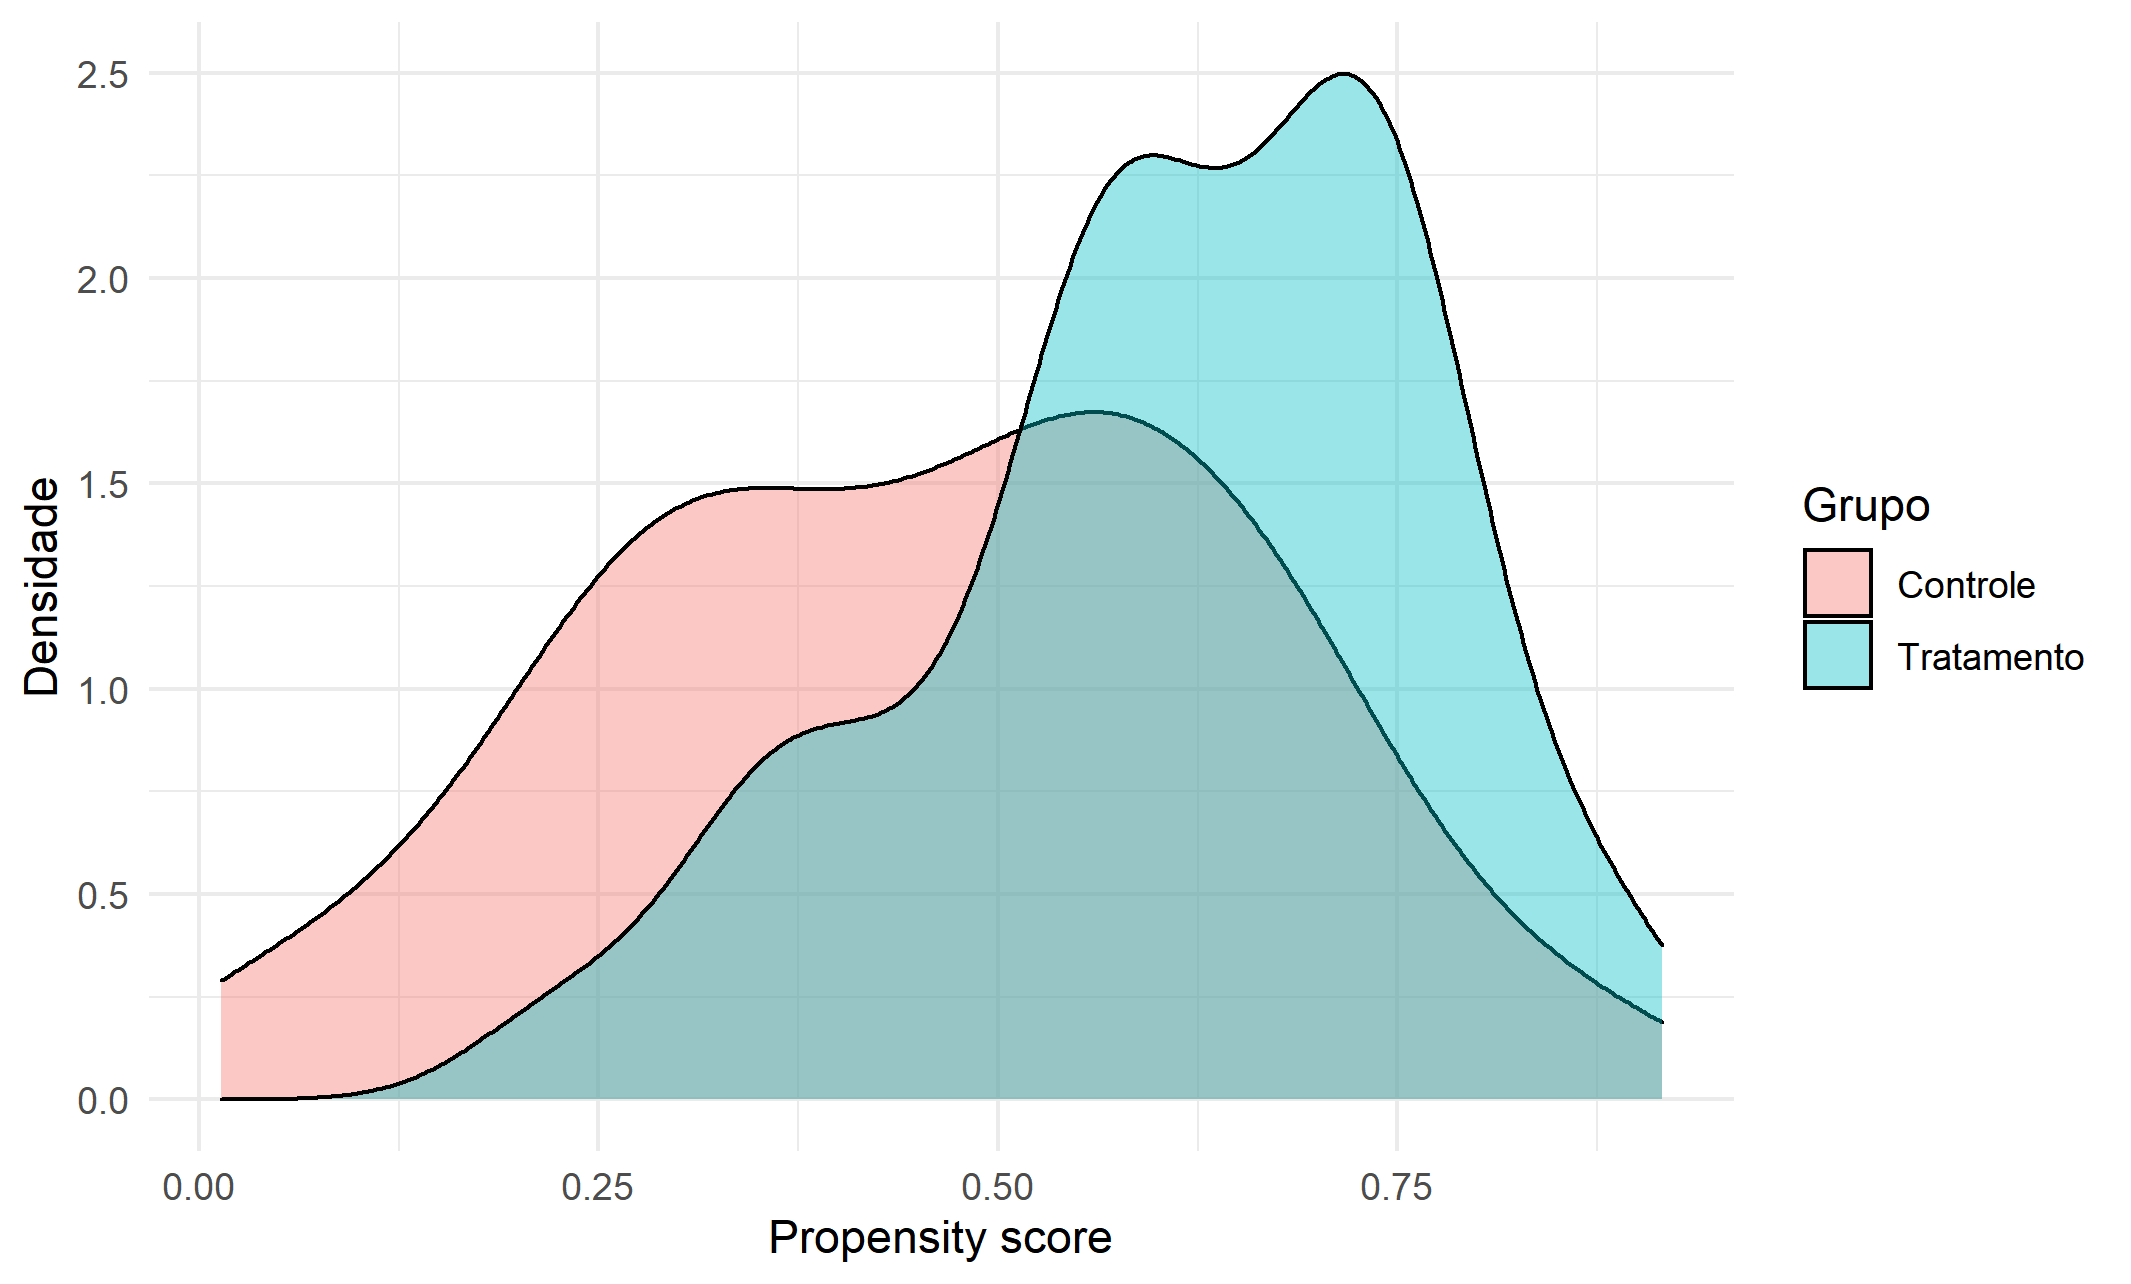
\includegraphics[width=0.7\linewidth]{"Figuras/suporte_comum_2009_2012.png"} \\
\caption*{\RaggedRight Fonte: Elaboração própria à partir dos Microdados do ENADE disponíveis em \cite{INEP2020}.}
\end{figure}

\begin{figure}[H]
	\centering
	\caption{Suporte comum - Ciclo 2010-2013 - PSM (logit)}
	\label{fig:suporte_comum_2010_2013}
	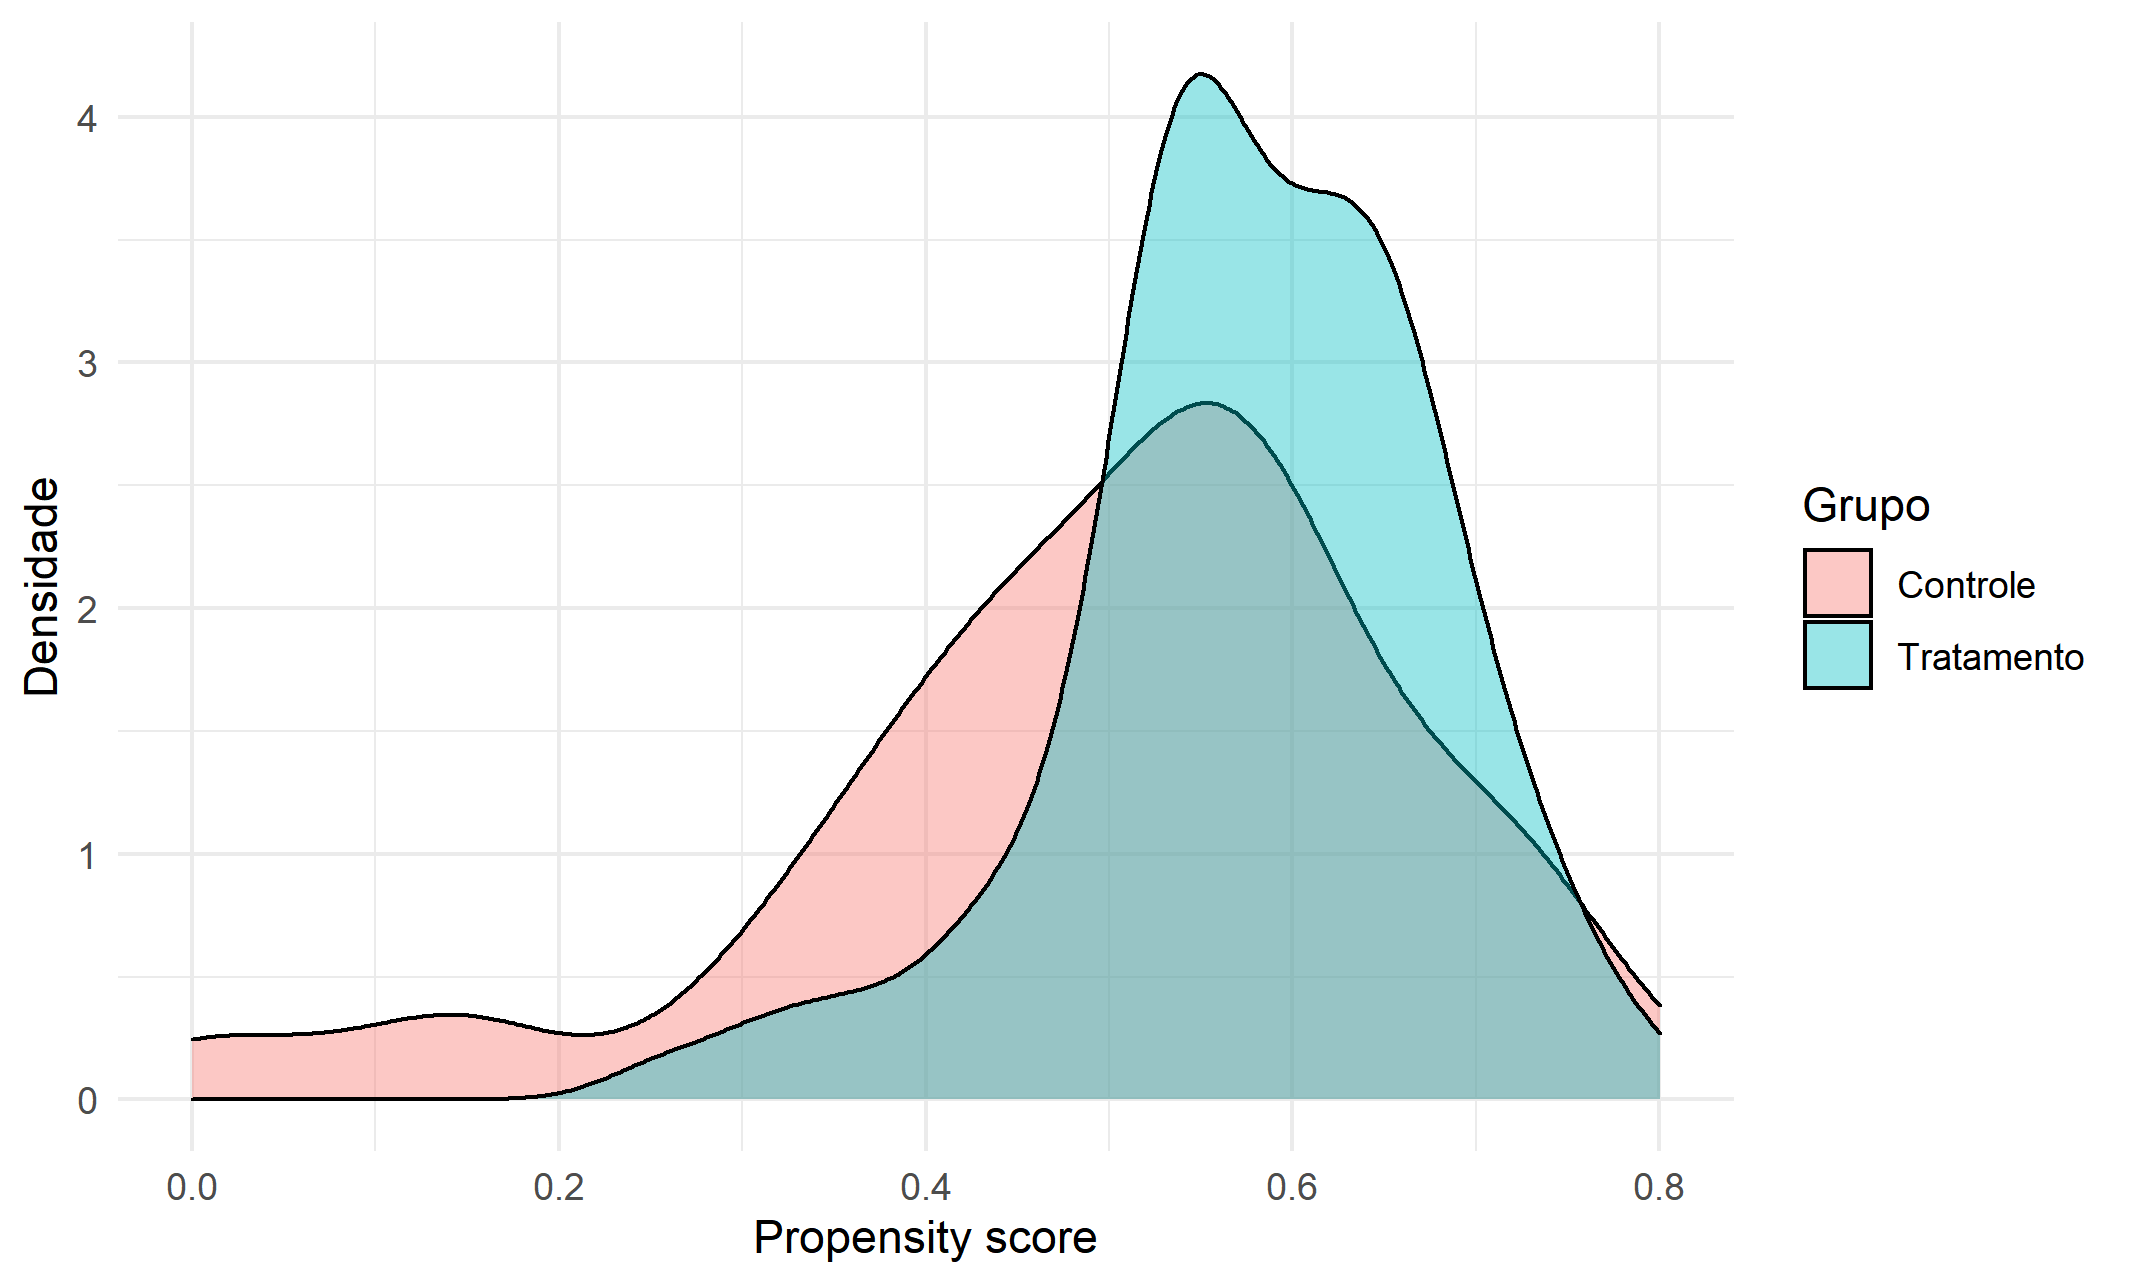
\includegraphics[width=0.7\linewidth]{"Figuras/suporte_comum_2010_2013.png"} \\
\caption*{\RaggedRight Fonte: Elaboração própria à partir dos Microdados do ENADE disponíveis em \cite{INEP2020}.}
\end{figure}

Em seguida, conforme recomendado em \citeonline{Garridoetal2014}, fez-se uma análise dessa mesma hipótese porém analisando agora os dados separados em quantis. Optou-se por utilizar cinco (5) quantis, sendo o último desses descartado devido ao pequeno número de observações (duas observações por grupo), ficando, portanto com quatro (4) quantis.

O resultado dessa divisão pode ser visualizado na Tabela \ref{tab:psm_quantil}, na qual tem-se o valor médio do PS em cada um dos quatro quantis para cada um dos grupos:

\begin{table}[H] \centering 
	\caption{Propensity score médio por quantil - Tratados x Controle} 
	\label{tab:psm_quantil} 
	\begin{tabular}{ccccc}
		\hline \hline Modelo & Quantil & Grupo & Propensity score  \\ \hline \\ \multirow{11}{*}{Ciclo 2009-2012} &  (0,014;0,4] & Controle & 0,251 \\ & (0,014;0,4] & Tratamento & 0,324 \\ \\ & (0,4;0,562] & Controle & 0,485 \\ & (0,4;0,562] & Tratamento & 0,507 \\ \\ & (0,562;0,69] & Controle & 0,625 \\ & (0,562;0,69] & Tratamento & 0,622 \\ \\ & (0,69;0,889] & Controle & 0,753 \\ & (0,69;0,889] & Tratamento & 0,756
		\\ \\ \hline \hline \\  \multirow{11}{*}{Ciclo 2010-2013} &  (0,000005;0,476] & Controle & 0,350 \\  & (0,000005;0,476] & Tratamento & 0,389 \\ \\ & (0,476;0,554] & Controle & 0,524  \\ & (0,476;0,554] & Tratamento & 0,526 \\ \\ & (0,554;0,632] & Controle & 0,586  \\ & (0,554;0,632] & Tratamento & 0,593 \\ \\ & (0,632;0,757] & Controle & 0,694  \\ & (0,632;0,757] & Tratamento & 0,675 \\ \\ \hline  \\
		\end{tabular}
		\caption*{\RaggedRight Fonte: Elaboração própria à partir dos Microdados do ENADE disponíveis em \cite{INEP2020}.}
	\end{table}

Note que para ambos os ciclos as médias são extremamente próximas, com as diferenças sendo em torno de 5\%, com exceção do primeiro quantil, que em ambas amostras se mostrou com a maior diferença relativa entre grupos. Apesar disso, considerou-se que a diferença não é grande o suficiente para ser um problema grave\footnote{Uma possibilidade de garantir ainda mais robustez aos resultados seria realizar uma estimação quantílica, separando, assim, o quantil "problemático" dos demais. Os autores do presente artigo crêem que a abordagem utilizada aqui é confiável o suficiente para ser útil.}.

Para corroborar essa hipótese, procedeu-se à construção de distribuições de densidade do PS para cada quantil, separados em grupo de tratamento e grupo de controle. Os resultados estão nas figuras \ref{fig:PSM_quantil_2009_2012} e \ref{fig:PSM_quantil_2010_2013}

\begin{figure}[H]
	\centering
	\caption{Suporte comum por quantil - Ciclo 2009-2012 - PSM (logit)}
	\label{fig:PSM_quantil_2009_2012}
	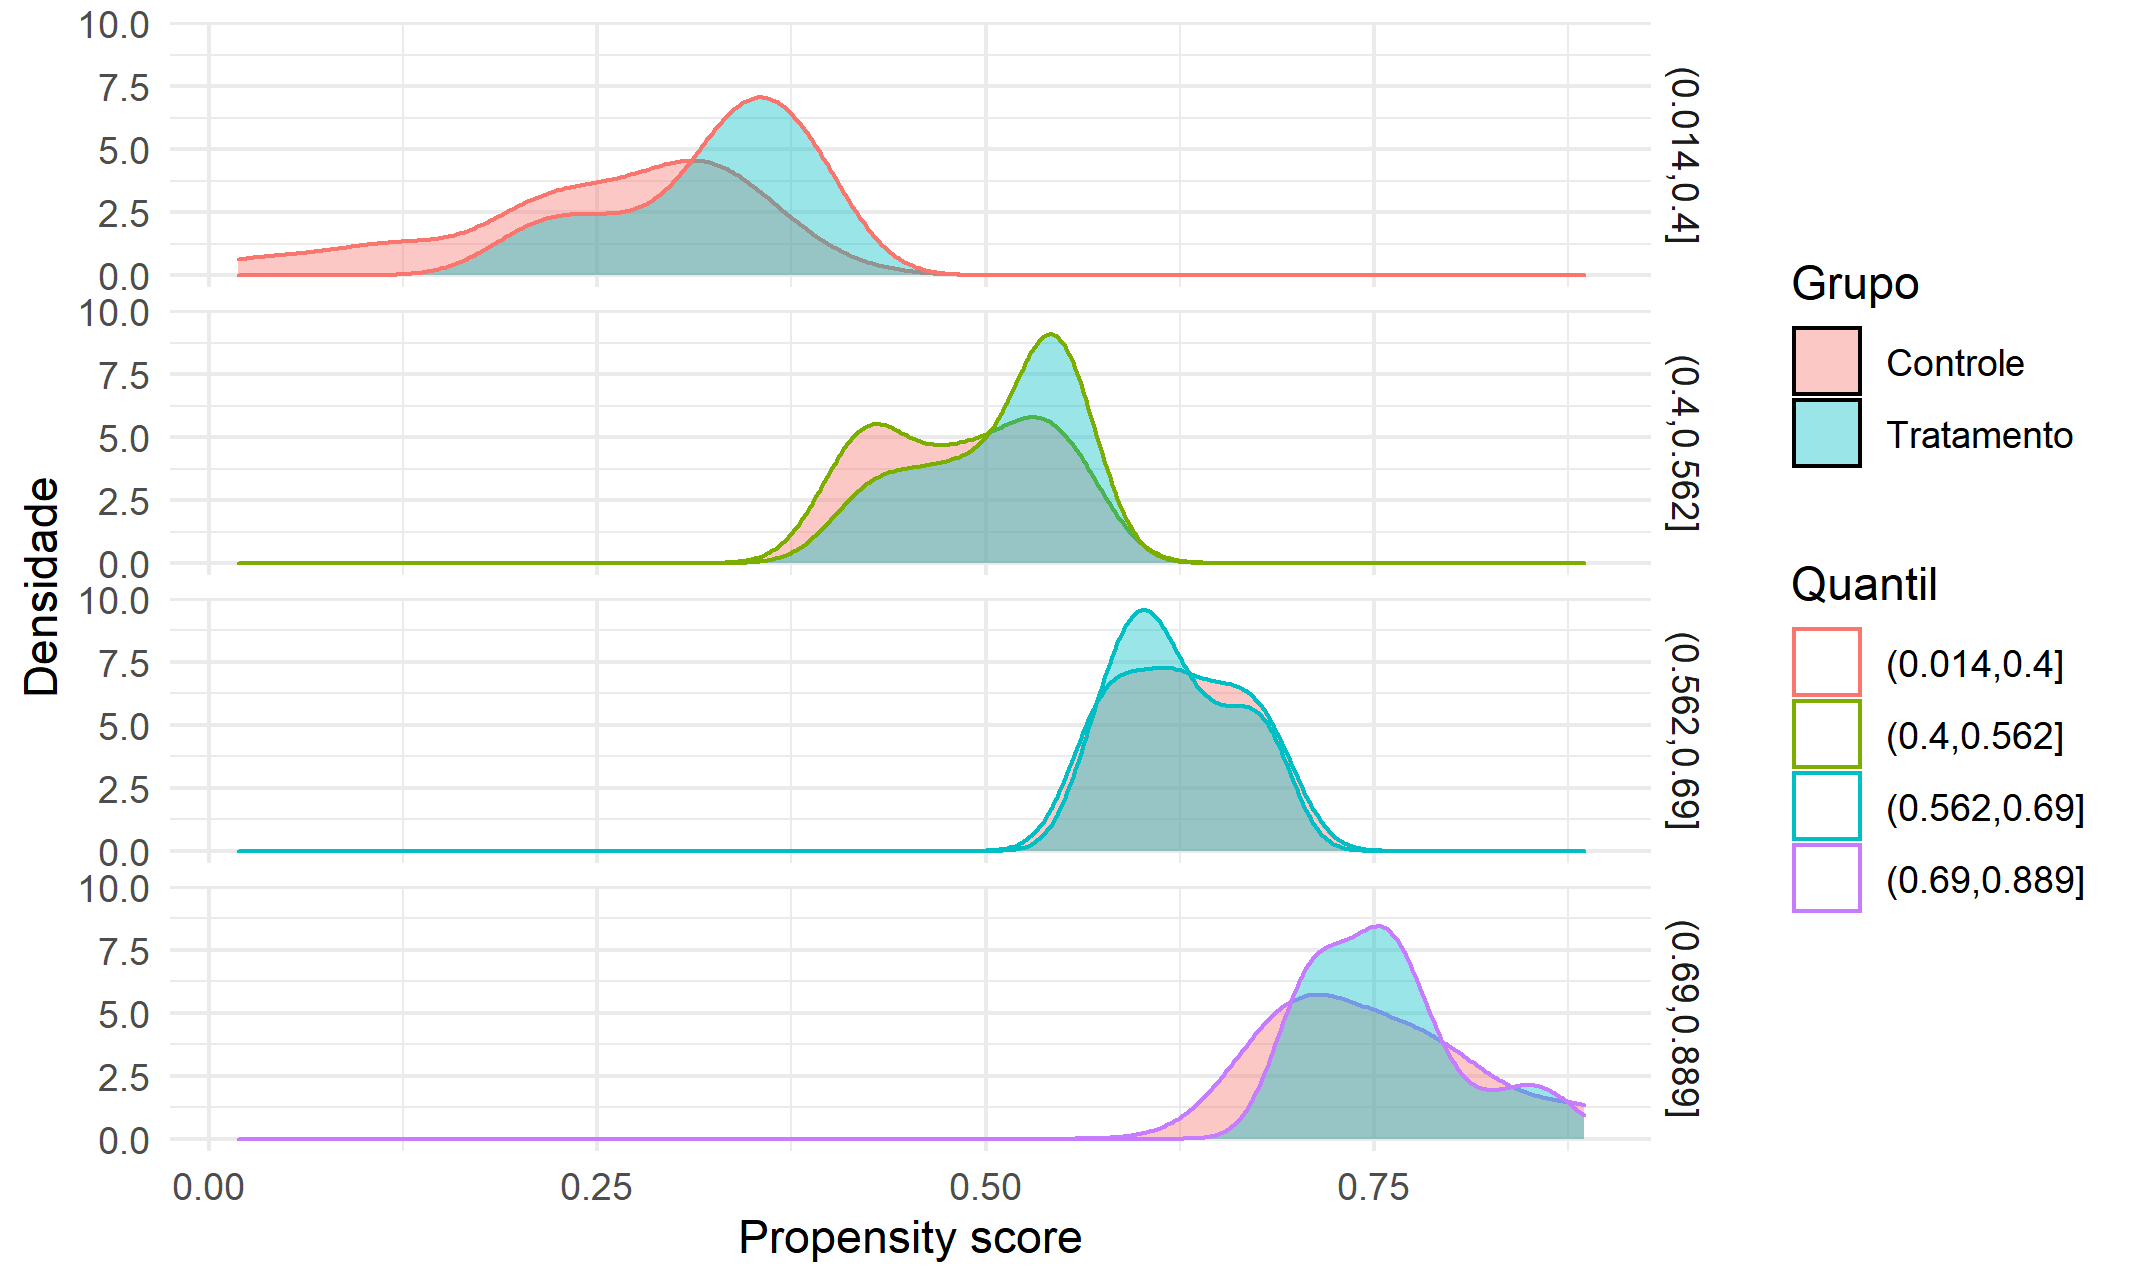
\includegraphics[width=0.7\linewidth]{"Figuras/suporte_comum_2009_2012_quantis.png"}
\caption*{\RaggedRight Fonte: Elaboração própria à partir dos Microdados do ENADE disponíveis em \cite{INEP2020}.}
\end{figure}

\begin{figure}[H]
	\centering
	\caption{Suporte comum por quantil - Ciclo 2010-2013 - PSM (logit)}
	\label{fig:PSM_quantil_2010_2013}
	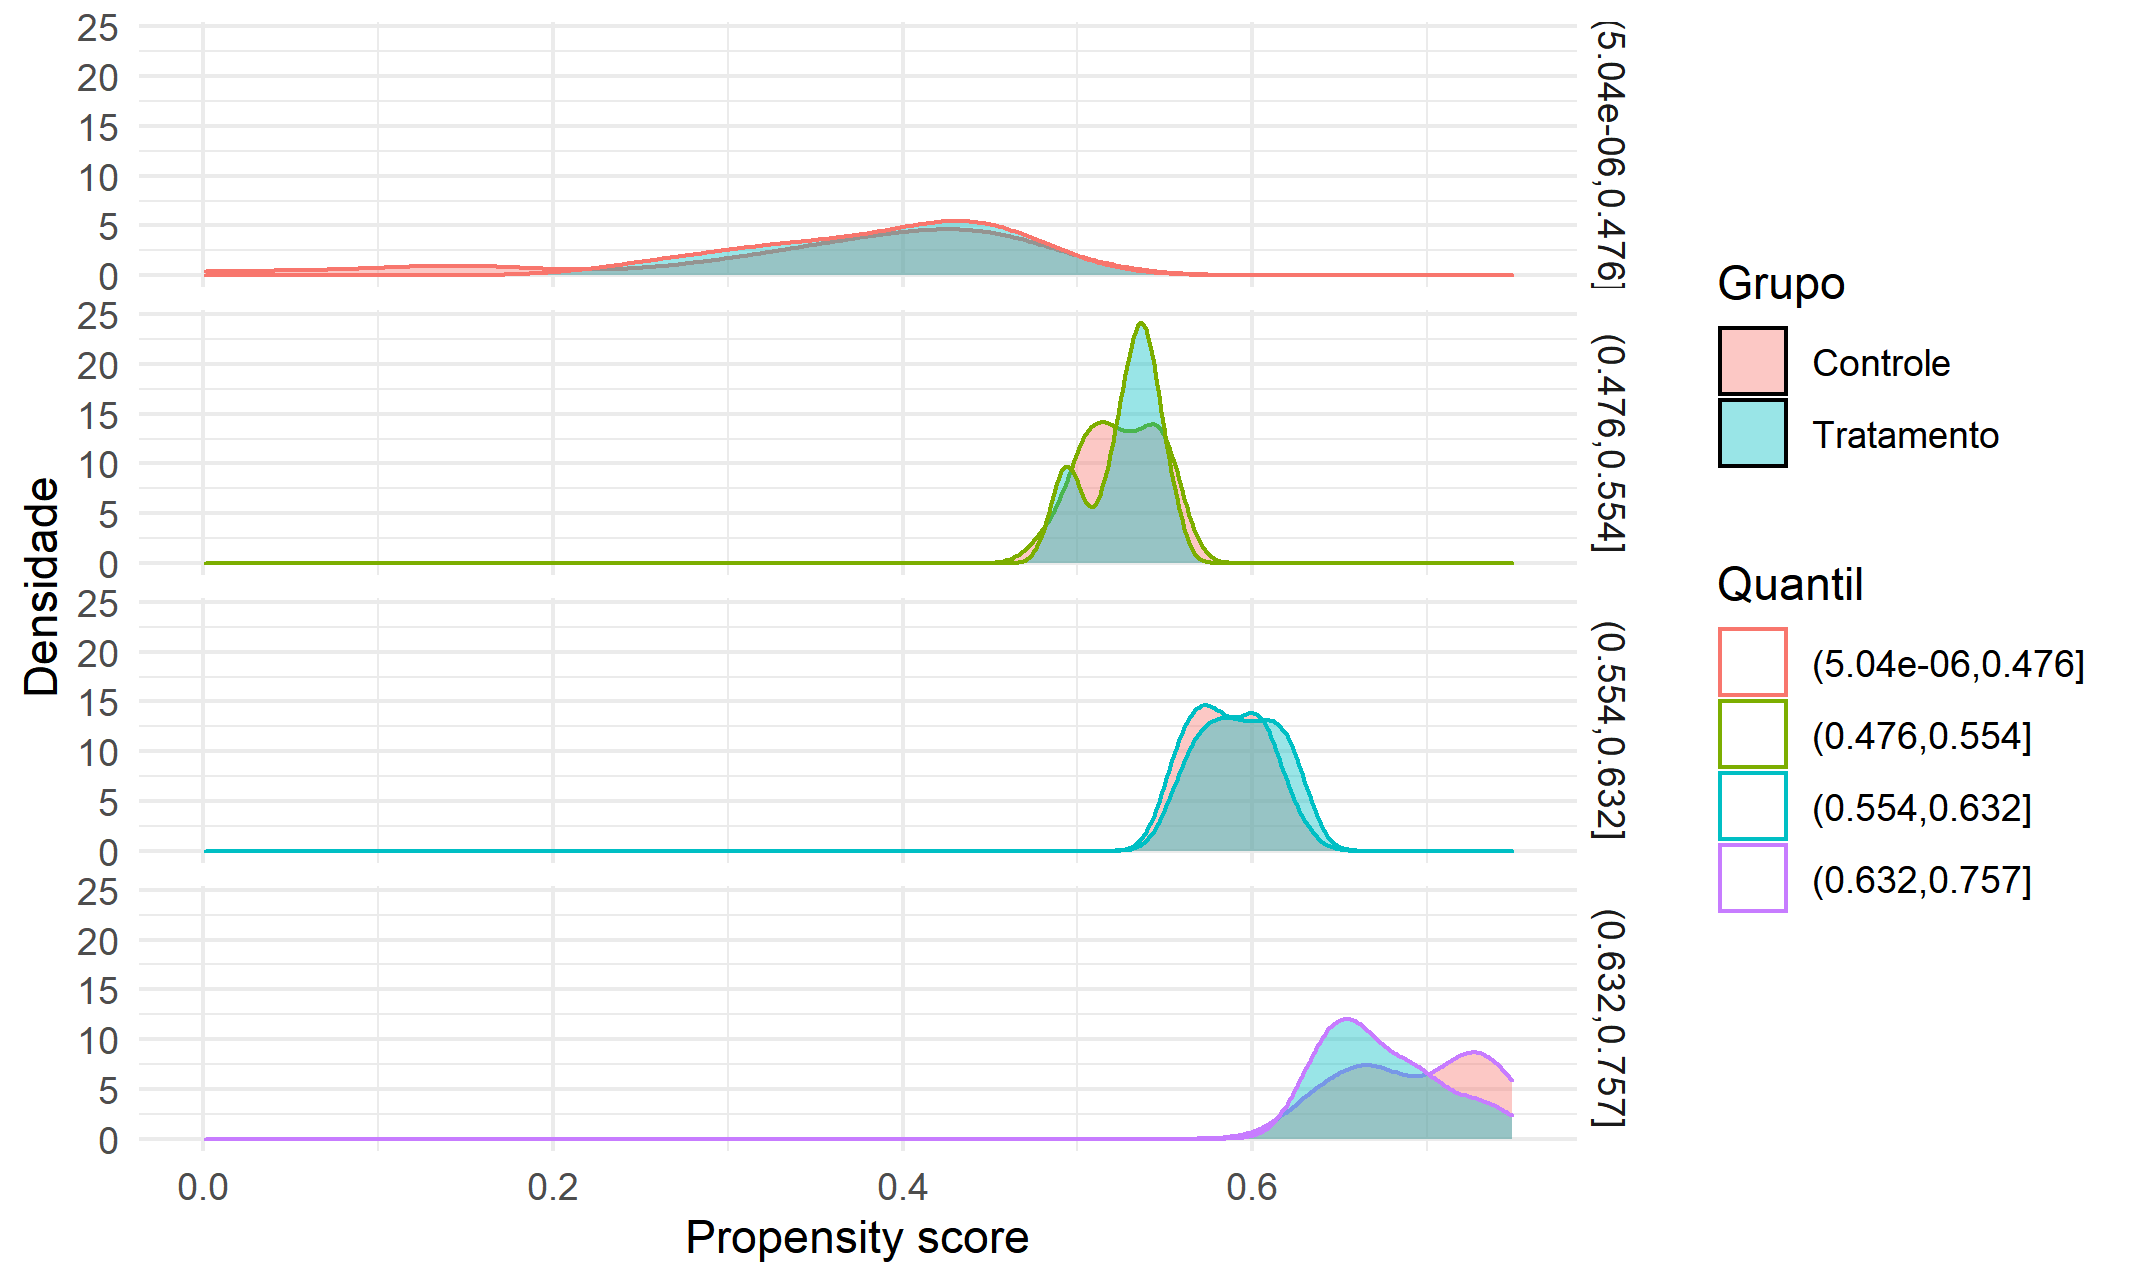
\includegraphics[width=0.7\linewidth]{"Figuras/suporte_comum_2010_2013_quantis.png"}
	\caption*{\RaggedRight Fonte: Elaboração própria à partir dos Microdados do ENADE disponíveis em \cite{INEP2020}.}
\end{figure}

De fato, vê-se que a análise visual apoia a hipótese da existência de suporte comum entre os grupos de tratamento e controle, ocorrendo isso até mesmo em nível de quartil. 

Na próxima seção, a análise do balanceamento das covariadas dos modelos, ou seja, do resultado da utilização do PSM, é realizada. Para tanto, foram utilizados gráficos que indicam, visualmente, como eram e como ficaram as diferenças entre as médias e a razão das variâncias de cada covariada entre os dois grupos.

\section{Balanceamento das covariadas}

Utilizando o comando \textit{love.plot} do pacote \textit{Cobalt} (\citeonline{Cobalt2020}) da linguagem \textit{R} (\citeonline{R2020}), criaram-se os diversos gráficos citados no parágrafo anterior. Eles encontram-se dispostos nas figuras \ref{fig:balanceamento_covariadas_2009_2012_probit}, \ref{fig:balanceamento_covariadas_2009_2012_entropia},\ref{fig:balanceamento_covariadas_2010_2013_probit} e \ref{fig:balanceamento_covariadas_2010_2013_entropia}.

\begin{figure}[H]
	\centering
	\caption{Balanceamento das covariadas - Ciclo 2009-2012 - PSM (logit)}
	\label{fig:balanceamento_covariadas_2009_2012_probit}
	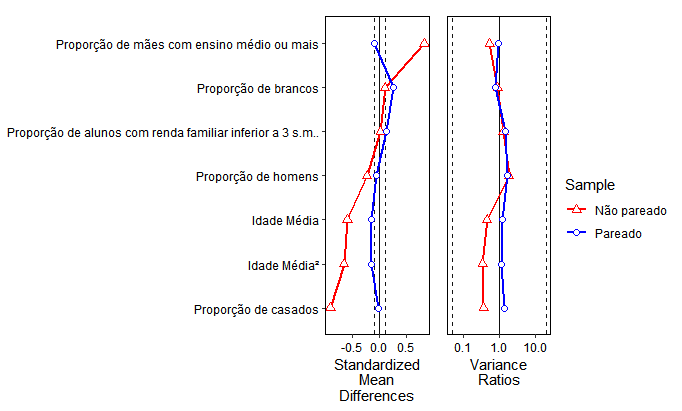
\includegraphics[width=0.7\linewidth]{"Figuras/balanceamento_covariadas_2009_2012_logit.png"}
	\caption*{\RaggedRight Fonte: Elaboração própria à partir dos Microdados do ENADE disponíveis em \cite{INEP2020}.}
\end{figure}

\begin{figure}[H]
	\centering
	\caption{Balanceamento das covariadas - Ciclo 2009-2012 - PSM (entropia)}
	\label{fig:balanceamento_covariadas_2009_2012_entropia}
	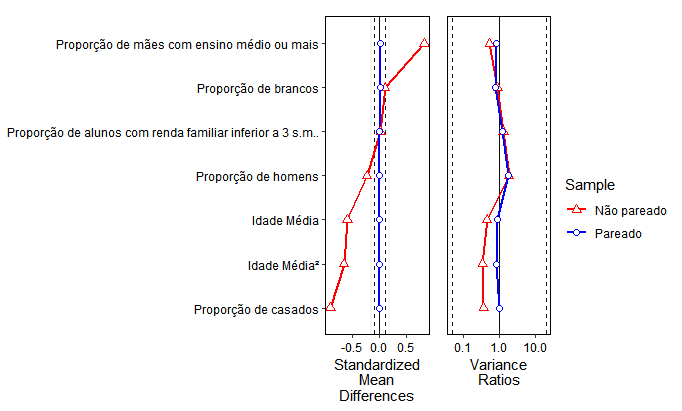
\includegraphics[width=0.7\linewidth]{"Figuras/balanceamento_covariadas_2009_2012_entropia.png"}
	\caption*{\RaggedRight Fonte: Elaboração própria à partir dos Microdados do ENADE disponíveis em \cite{INEP2020}.}
\end{figure}


\begin{figure}[H]
	\centering
	\caption{Balanceamento das covariadas - Ciclo 2010-2013 - PSM (logit)}
	\label{fig:balanceamento_covariadas_2010_2013_probit}
	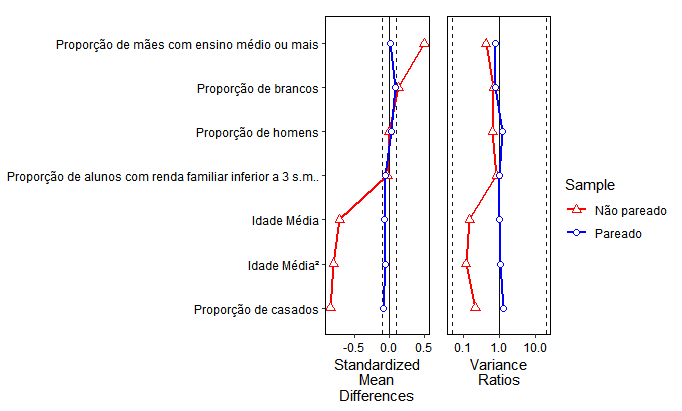
\includegraphics[width=0.7\linewidth]{"Figuras/balanceamento_covariadas_2010_2013_logit.png"}
	\caption*{\RaggedRight Fonte: Elaboração própria à partir dos Microdados do ENADE disponíveis em \cite{INEP2020}.}
\end{figure}


\begin{figure}[H]
	\centering
	\caption{Balanceamento das covariadas - Ciclo 2010-2013 - PSM (entropia)}
	\label{fig:balanceamento_covariadas_2010_2013_entropia}
	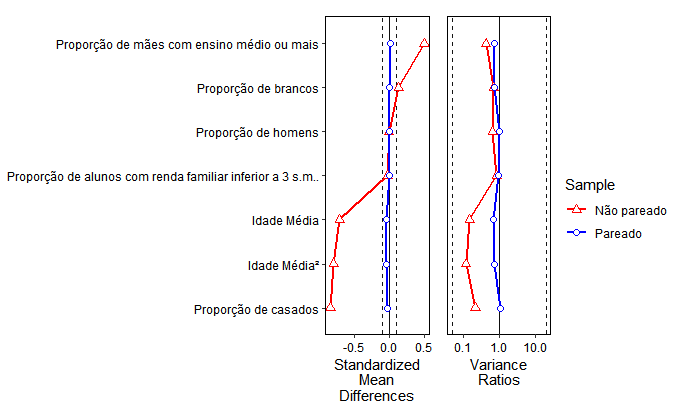
\includegraphics[width=0.7\linewidth]{"Figuras/balanceamento_covariadas_2010_2013_entropia.png"}
	\caption*{\RaggedRight Fonte: Elaboração própria à partir dos Microdados do ENADE disponíveis em \cite{INEP2020}.}
\end{figure}

Notadamente, como se pode perceber em todas as figuras, os grupos eram muito diferentes entre si, com quase nenhuma das variáveis tendo médias semelhantes, embora suas variâncias fossem parecidas. Apesar disso, os métodos empregados tiveram sucesso em tornar os dois grupos comparáveis.

Veja que até o ajuste relativamente menos complexo realizado pelo PSM com \textit{logit} já conseguiu praticamente zerar as diferenças entre médias e variâncias em ambos os ciclos. Não obstante, a utilização do cálculo de \textbf{entropia} serviu para melhorar ainda mais os resultados, conseguindo deixar praticamente todas as variáveis dentro dos limiares aceitáveis tradicionais.

Na próxima seção é tratada a hipótese crucial do modelo de Diferenças-em-Diferenças (DD), a saber, a de que a variável de interesse tem trajetória igual (ou próxima) para ambos os grupos antes do tratamento. Para isso, foi utilizada uma inspeção gráfica, bem como a estimação de dois modelos de placebo. 

\subsection{Diferenças em diferenças}

\subsubsection{Tendências paralelas - inspeção gráfica}

Iniciando a análise com uma inspeção ingênua, puramente gráfica, tem-se a figura \ref{fig:tendencias}

\begin{figure}[H]
	\centering
	\caption{Tendências temporais - Nota média por grupo de tratamento}
	\label{fig:tendencias}
	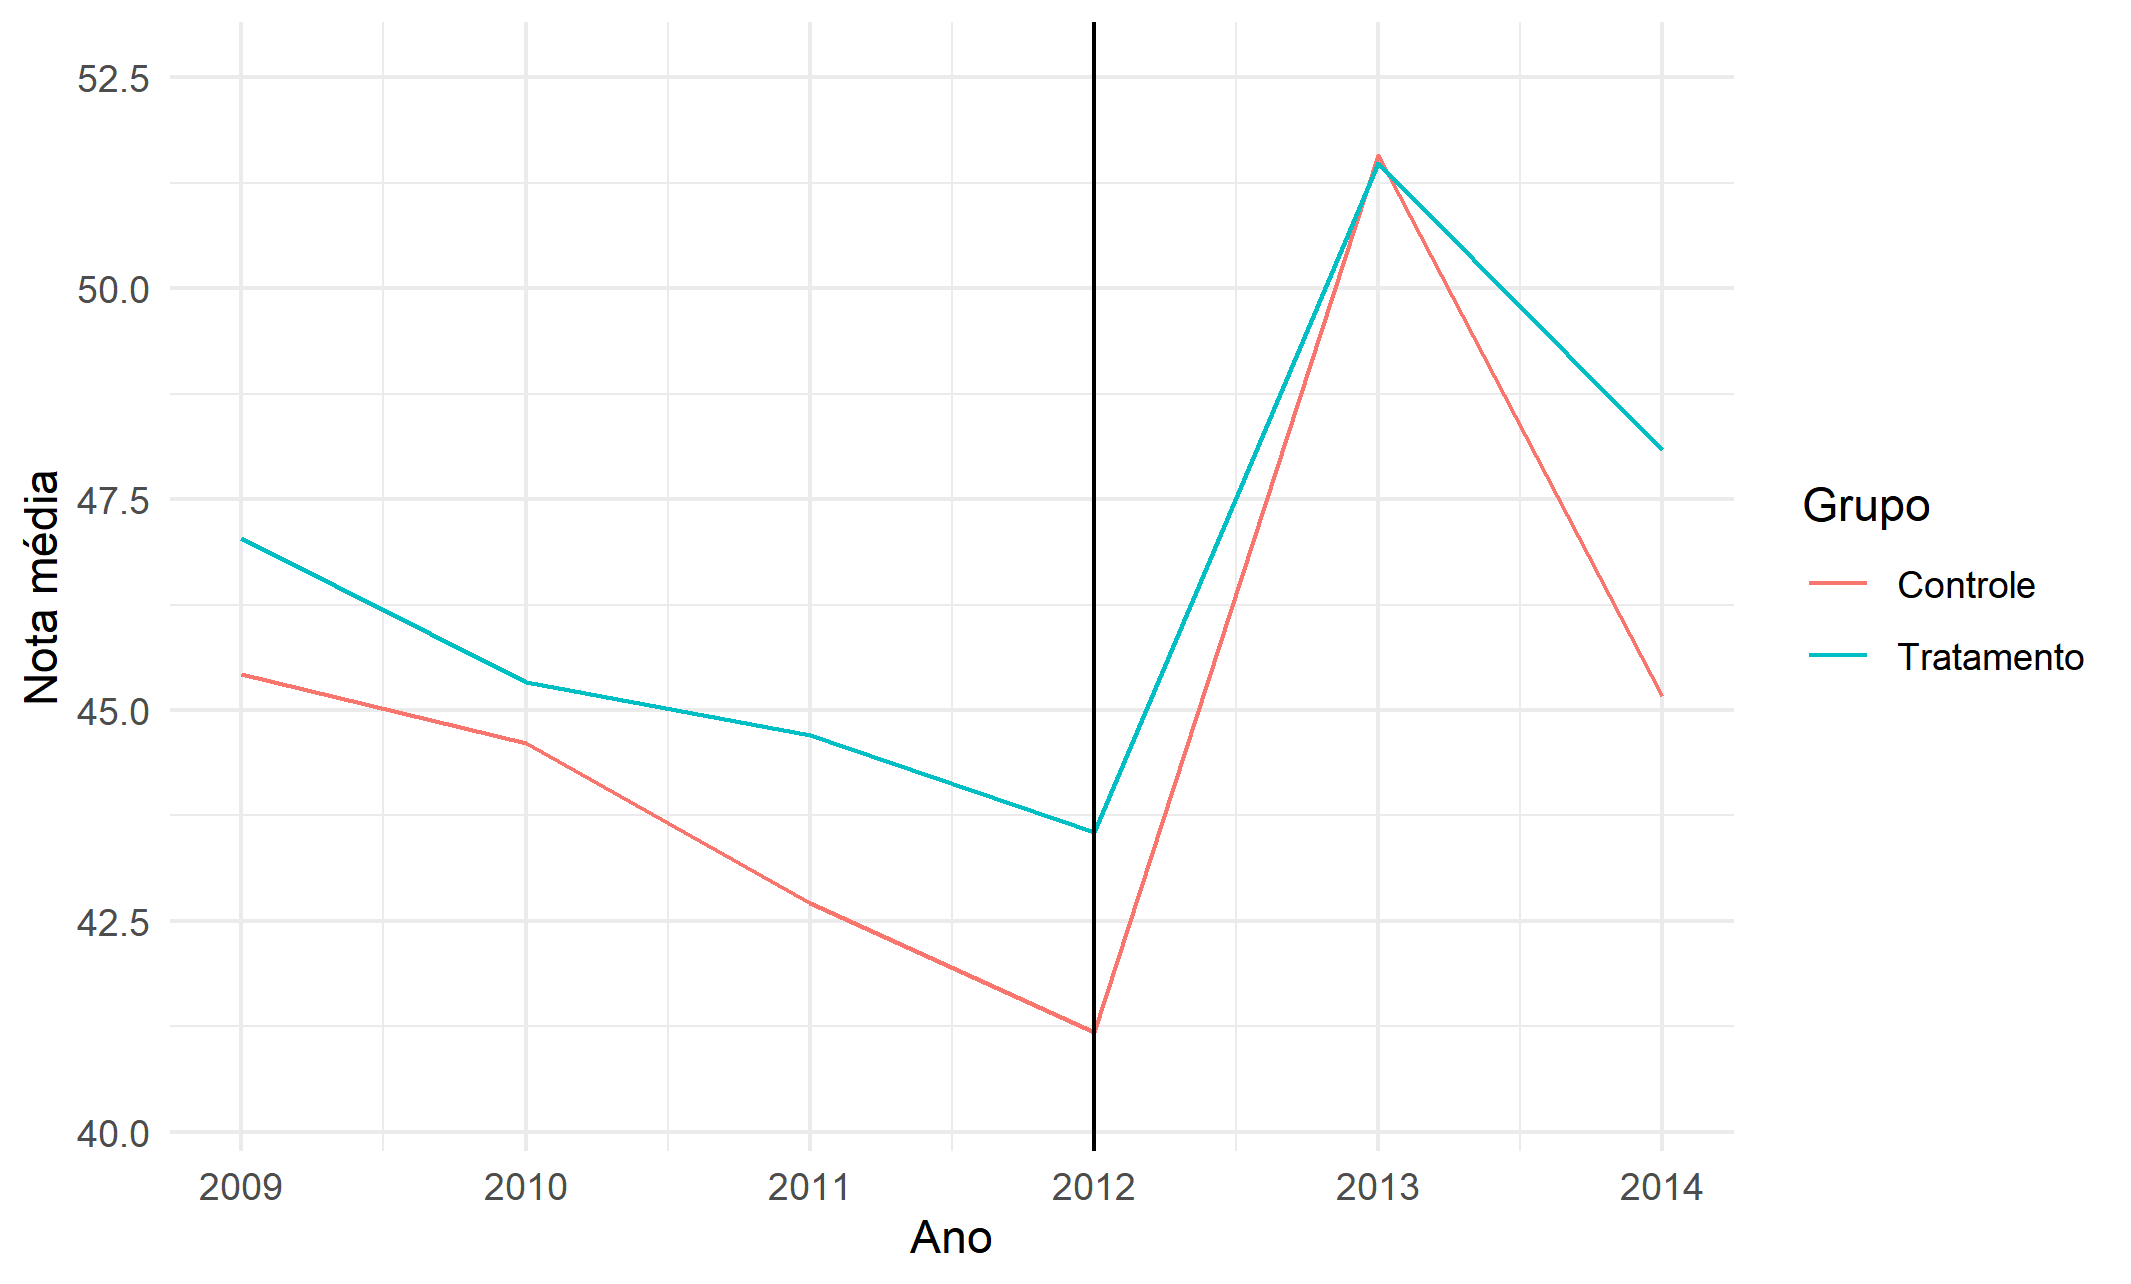
\includegraphics[width=0.7\linewidth]{"Figuras/tendencias.png"} \\
	\caption*{\RaggedRight Fonte: Elaboração própria à partir dos Microdados do ENADE disponíveis em \cite{INEP2020}.}
\end{figure}

Note que ao menos visualmente a trajetória para ambos os grupos é \textbf{muito próxima}, indicando que possivelmente o \textit{matching} teve sucesso e temos resultados confiáveis. A seguir tratará-se da estimação de dois modelos placebos para cada ciclo: o primeiro, considerando a proporção de casados como variável dependente, e o segundo, tratando a educação da mãe como variável dependente. Como já foi abordado, espera-se que o tratamento não tenha efeito sobre essas variáveis, o que indicaria que não houve nenhum choque no período que possa ter feito com que as trajetórias se desviassem.

\subsubsection{Teste de placebo}

Nas tabelas \ref{tab:placebo_2009_2012} e \ref{tab:placebo_2010_2013}, têm-se o resultado das estimações dos modelos de placebo.\footnote{Por uma questão de espaço, optou-se por colocar os gráficos de análise de balanceamento dos testes de placebo no apêndice. Esteja seguro, entretanto, de que todos os \textit{matchings} obtiveram sucesso.}

\begin{table}[H] \centering 
  \caption{Placebo - Ciclo 2009-2012} 
  \label{tab:placebo_2009_2012} 
\small 
\begin{tabular}{@{\extracolsep{5pt}}lD{,}{,}{-3} D{,}{,}{-3} } 
\\[-1.8ex]\hline 
\hline \\[-1.8ex] 
 & \multicolumn{2}{c}{\textit{Variável dependente:}} \\ 
\cline{2-3} 
\\[-1.8ex] & \multicolumn{1}{c}{Proporção de casados} & \multicolumn{1}{c}{Proporção de mães com ensino médio+} \\ \cline{2-3} 
\hline \\[-1.8ex] 
 Pós-tratamento & -0,037^{***} & 0,079^{***} \\ 
  & (0,009) & (0,016) \\ 
  & & \\ 
 Idade média & -0,008 & -0,018 \\ 
  & (0,018) & (0,034) \\ 
  & & \\ 
 Idade média² & 0,001^{*} & -0,0003 \\ 
  & (0,0004) & (0,001) \\ 
  & & \\ 
 Prop. brancos & 0,096 & 0,238 \\ 
  & (0,080) & (0,153) \\ 
  & & \\ 
 Prop. casados &  & -0,175 \\ 
  &  & (0,219) \\ 
  & & \\ 
 Nota média & -0,001^{*} & 0,001 \\ 
  & (0,001) & (0,001) \\ 
  & & \\ 
 Prop. renda até 3SM & 0,006  & -0,082 \\ 
  & (0,030) & (0,058) \\ 
  & & \\ 
 Prop. homens & 0,019 & 0,023 \\ 
  & (0,044) & (0,082) \\ 
  & & \\ 
 Prop. Ensino Médio+ & -0,049 &  \\ 
  & (0,060) &  \\ 
  & & \\ 
 Diff-and-diff/Impacto & -0,001 & 0,011 \\ 
  & (0,006) & (0,011) \\ 
  & & \\ 
\hline \\[-1.8ex] 
Observações & \multicolumn{1}{c}{170} & \multicolumn{1}{c}{170} \\ 
Estatística F (df = 9; 76) & \multicolumn{1}{c}{28,765$^{***}$} & \multicolumn{1}{c}{10,020$^{***}$} \\ 
\hline 
\hline \\[-1.8ex] 
\textit{Nota¹:}  & \multicolumn{2}{r}{$^{*}$p$<$0,1; $^{**}$p$<$0,05; $^{***}$p$<$0,01} \\ \textit{Nota²:} & \multicolumn{2}{r}{Os dois modelos foram estimados utilizando DD+FE+PSM (entropia) } \\ \hline
\end{tabular} \\
\caption*{\RaggedRight Fonte: Elaboração própria à partir dos Microdados do ENADE disponíveis em \cite{INEP2020}.}
\end{table} 


\begin{table}[H] \centering 
  \caption{Placebo - Ciclo 2010-2013} 
  \label{tab:placebo_2010_2013} 
\small 
\begin{tabular}{@{\extracolsep{5pt}}lD{,}{,}{-3} D{,}{,}{-3} } 
\\[-1.8ex]\hline 
\hline \\[-1.8ex] 
 & \multicolumn{2}{c}{\textit{Variável dependente:}} \\ 
\cline{2-3} 
\\[-1.8ex] & \multicolumn{1}{c}{Proporção de casados} & \multicolumn{1}{c}{Proporção de mães com ensino médio+} \\ 
\hline \\[-1.8ex] 
 Pós-tratamento & -0,035^{**} & 0,041 \\ 
  & (0,015) & (0,046) \\ 
  & & \\ 
 Idade média & -0,004 & -0,126 \\ 
  & (0,030) & (0,078) \\ 
  & & \\ 
 Idade média² & 0,0005 & 0,002 \\ 
  & (0,001) & (0,002) \\ 
  & & \\ 
 Prop. brancos & 0,008 & 0,751^{***} \\ 
  & (0,046) & (0,103) \\ 
  & & \\ 
 Prop. casados &  & 0,191 \\ 
  &  & (0,335) \\ 
  & & \\ 
 Nota média & -0,001 & 0,006^{***} \\ 
  & (0,001) & (0,002) \\ 
  & & \\ 
 Prop. renda até 3SM & 0,078^{***} & 0,143^{*} \\ 
  & (0,026) & (0,075) \\ 
  & & \\ 
 Prop. homens & -0,129^{**} & -0,037 \\ 
  & (0,052) & (0,170) \\ 
  & & \\ 
 Prop. Ensino Médio+ & 0,026 &  \\ 
  & (0,039) &  \\ 
  & & \\ 
 Diff-and-diff/Impacto & 0,003 & 0,034^{*} \\ 
  & (0,006) & (0,018) \\ 
  & & \\ 
\hline \\[-1.8ex] 
Observações & \multicolumn{1}{c}{170} & \multicolumn{1}{c}{170} \\ 
Estatística F (df = 9; 76) & \multicolumn{1}{c}{36,792$^{***}$} & \multicolumn{1}{c}{38,078$^{***}$} \\ 
\hline 
\hline \\[-1.8ex] 
\textit{Nota¹:}  & \multicolumn{2}{r}{$^{*}$p$<$0,1; $^{**}$p$<$0,05; $^{***}$p$<$0,01} \\ \textit{Nota²:} & \multicolumn{2}{r}{Os dois modelos foram estimados utilizando DD+FE+PSM (entropia)} \\ \hline
\end{tabular}  \\
\caption*{\RaggedRight Fonte: Elaboração própria à partir dos Microdados do ENADE disponíveis em \cite{INEP2020}.}
\end{table} 

Veja que em três (3) dos quatro (4) modelos estimados, a variável de impacto não teve significância estatística. Uma possível explicação para a variável ter sido significativa no último modelo é que, em alguma medida, os alunos com mães que têm maior nível de educação participaram menos, relativamente, das provas do ENADE 2013, do que os demais discentes em razão da greve. Apesar disso, o problema não parece causar nada muito grave e podemos concluir pela validade da nossa estimação de placebo.

Findada a apresentação das medidas tomadas para garantir a robustez dos resultados obtidos, na próxima subseção eles são apresentados e discutidos. 

\section{Análise de impacto}

Inicialmente foi feita a análise dos resultados obtidos para o Ciclo 2009-2012 e depois para o Ciclo 2010-2013. A tabela \ref{tab:resultados_2009_2012} apresenta as estimações realizadas para o primeiro Ciclo. 

Nota-se que as variáveis já consagradas na literatura têm os sinais esperados e são significativas: a idade é positivamente correlacionada com a nota, apresentando, entretanto, concavidade, indicando que seu efeito é decrescente no tempo. A proporção de estudantes com renda familiar de até três (3) salários tem relação negativa com a nota, possivelmente pela melhor educação que o dinheiro pode proporcionar. 

A variável que captura a proporção de casados nas instituições é estatisticamente significativa e apresenta relação negativa com a nota. Uma possível razão para isso é que discentes casados têm menos tempo para dedicarem aos seus estudos, o que se traduziria em uma nota menor para esse grupo.

É importante frisar como os resultados mudam, se comparados o modelo ingênuo de DD com o modelo final, mais roubusto, de DD + FE + PSM (entropia). A variável que captura a proporção de brancos em cada IES muda de sinal e aumenta expressivamente em magnitude, indicando que uma maior proporção de brancos é negativamente correlacionada com a nota média da instituição. 

A variável de impacto, entretanto, não ganha significância. Seu coeficiente aponta uma relação positiva com a nota média. Possivelmente a variável não foi significativa pois os maiores efeitos da greve levam um certo intervalo de tempo para serem sentidos, hipótese que é retomada na discussão a seguir. Supondo que ela fosse significativa nesse ciclo, a distribuição de seu efeito marginal ao longo das observações, considerando apenas o modelo mais robusto, seria como está representado na figura \ref{fig:Efeitos_marginais_2009_2012}\footnote{No caso do modelo log-lin estimado, o efeito marginal não é linear e depende do valor da variável dependente.}, onde a linha vertical representa o limiar de ocorrência da intervenção.

\begin{figure}[H]
	\centering
	\caption{Efeitos marginais da variável de impacto - Ciclo 2009-2012}
	\label{fig:Efeitos_marginais_2009_2012}
	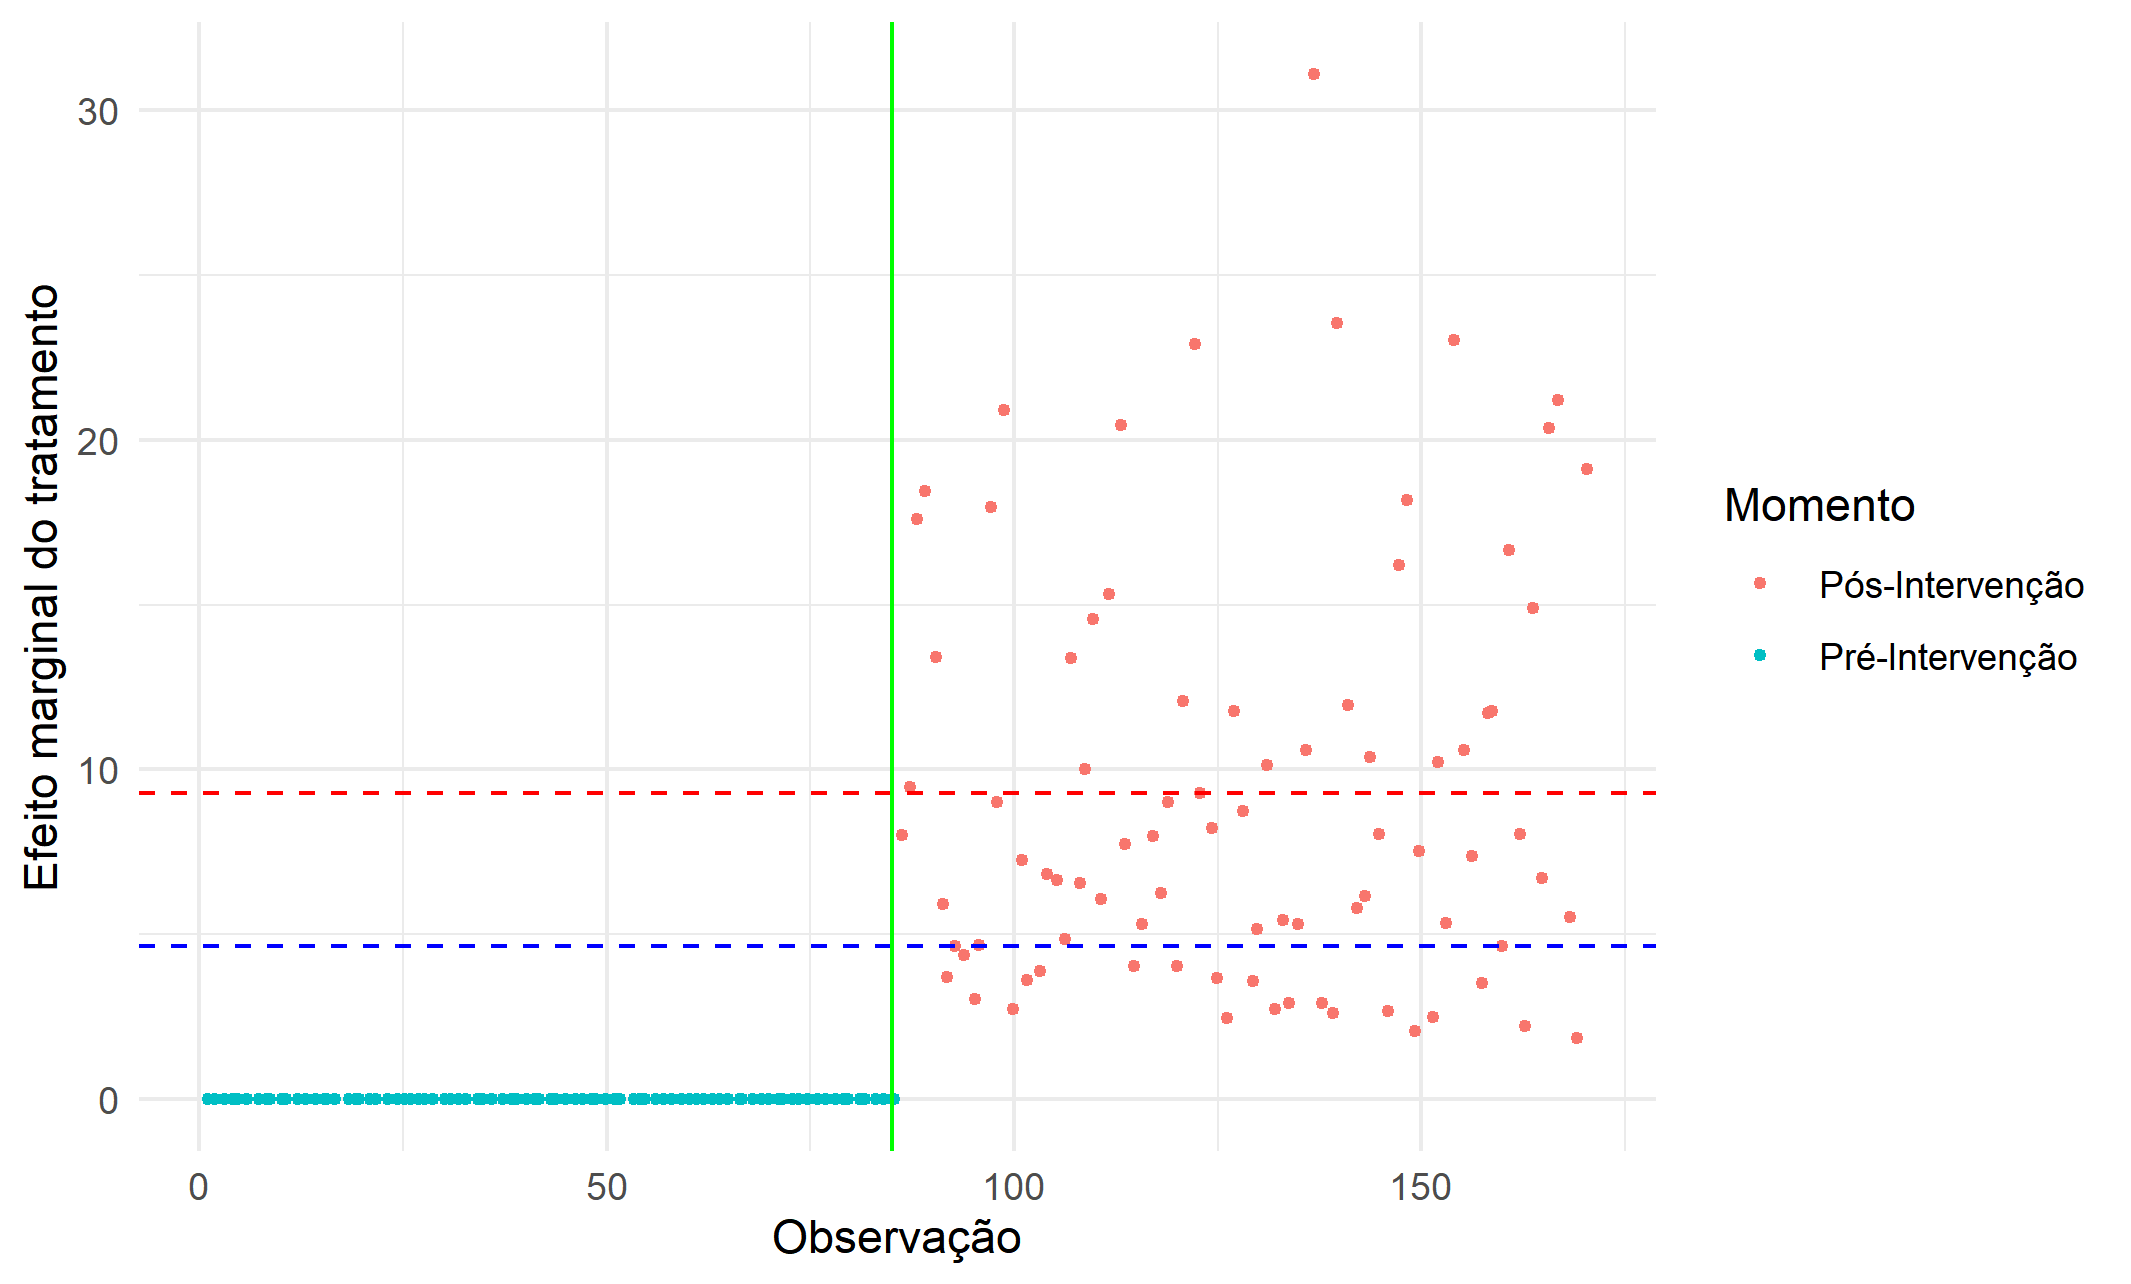
\includegraphics[width=0.7\linewidth]{"Figuras/Efeitos_marginais_2009_2012.png"} \\
\caption*{\RaggedRight Fonte: Elaboração própria à partir dos Microdados do ENADE disponíveis em \cite{INEP2020}.}
\end{figure}

Fazendo agora a análise dos resultados para o segundo ciclo, cujas estimações encontram-se na tabela \ref{tab:resultados_2010_2013}, tem-se que muita coisa mudou. Todas as variáveis perderam significância, com exceção da variável de impacto. Entretanto, seu sinal se inverteu, indicando que a greve teve um efeito de longo-prazo sobre os rendimentos dos alunos. Isso faz sentido, quando se considera o impacto que as greves tiveram sobre os calendários acadêmicos subsequentes. Esse resultado é semelhante ao obtido por \citeonline{Annegues2017}, que encontraram que as greves tiveram um impacto negativo estatisticamente significativo sobre o desempenho dos discentes da Universidade Federal da Paraíba (UFPB) em seus respectivos cursos, medidos pelas suas notas.

Em magnitude, o efeito marginal médio da variável de impacto foi de uma redução de $0,3798$ na nota média das instituições, considerando o período pós-greve ($t = 1$). A distribuição de seu efeito marginal ao longo das observações é como está representada na figura \ref{fig:Efeitos_marginais_2010_2013}

\begin{figure}[H]
	\centering
	\caption{Efeitos marginais da variável de impacto - Ciclo 2010-2013}
	\label{fig:Efeitos_marginais_2010_2013}
	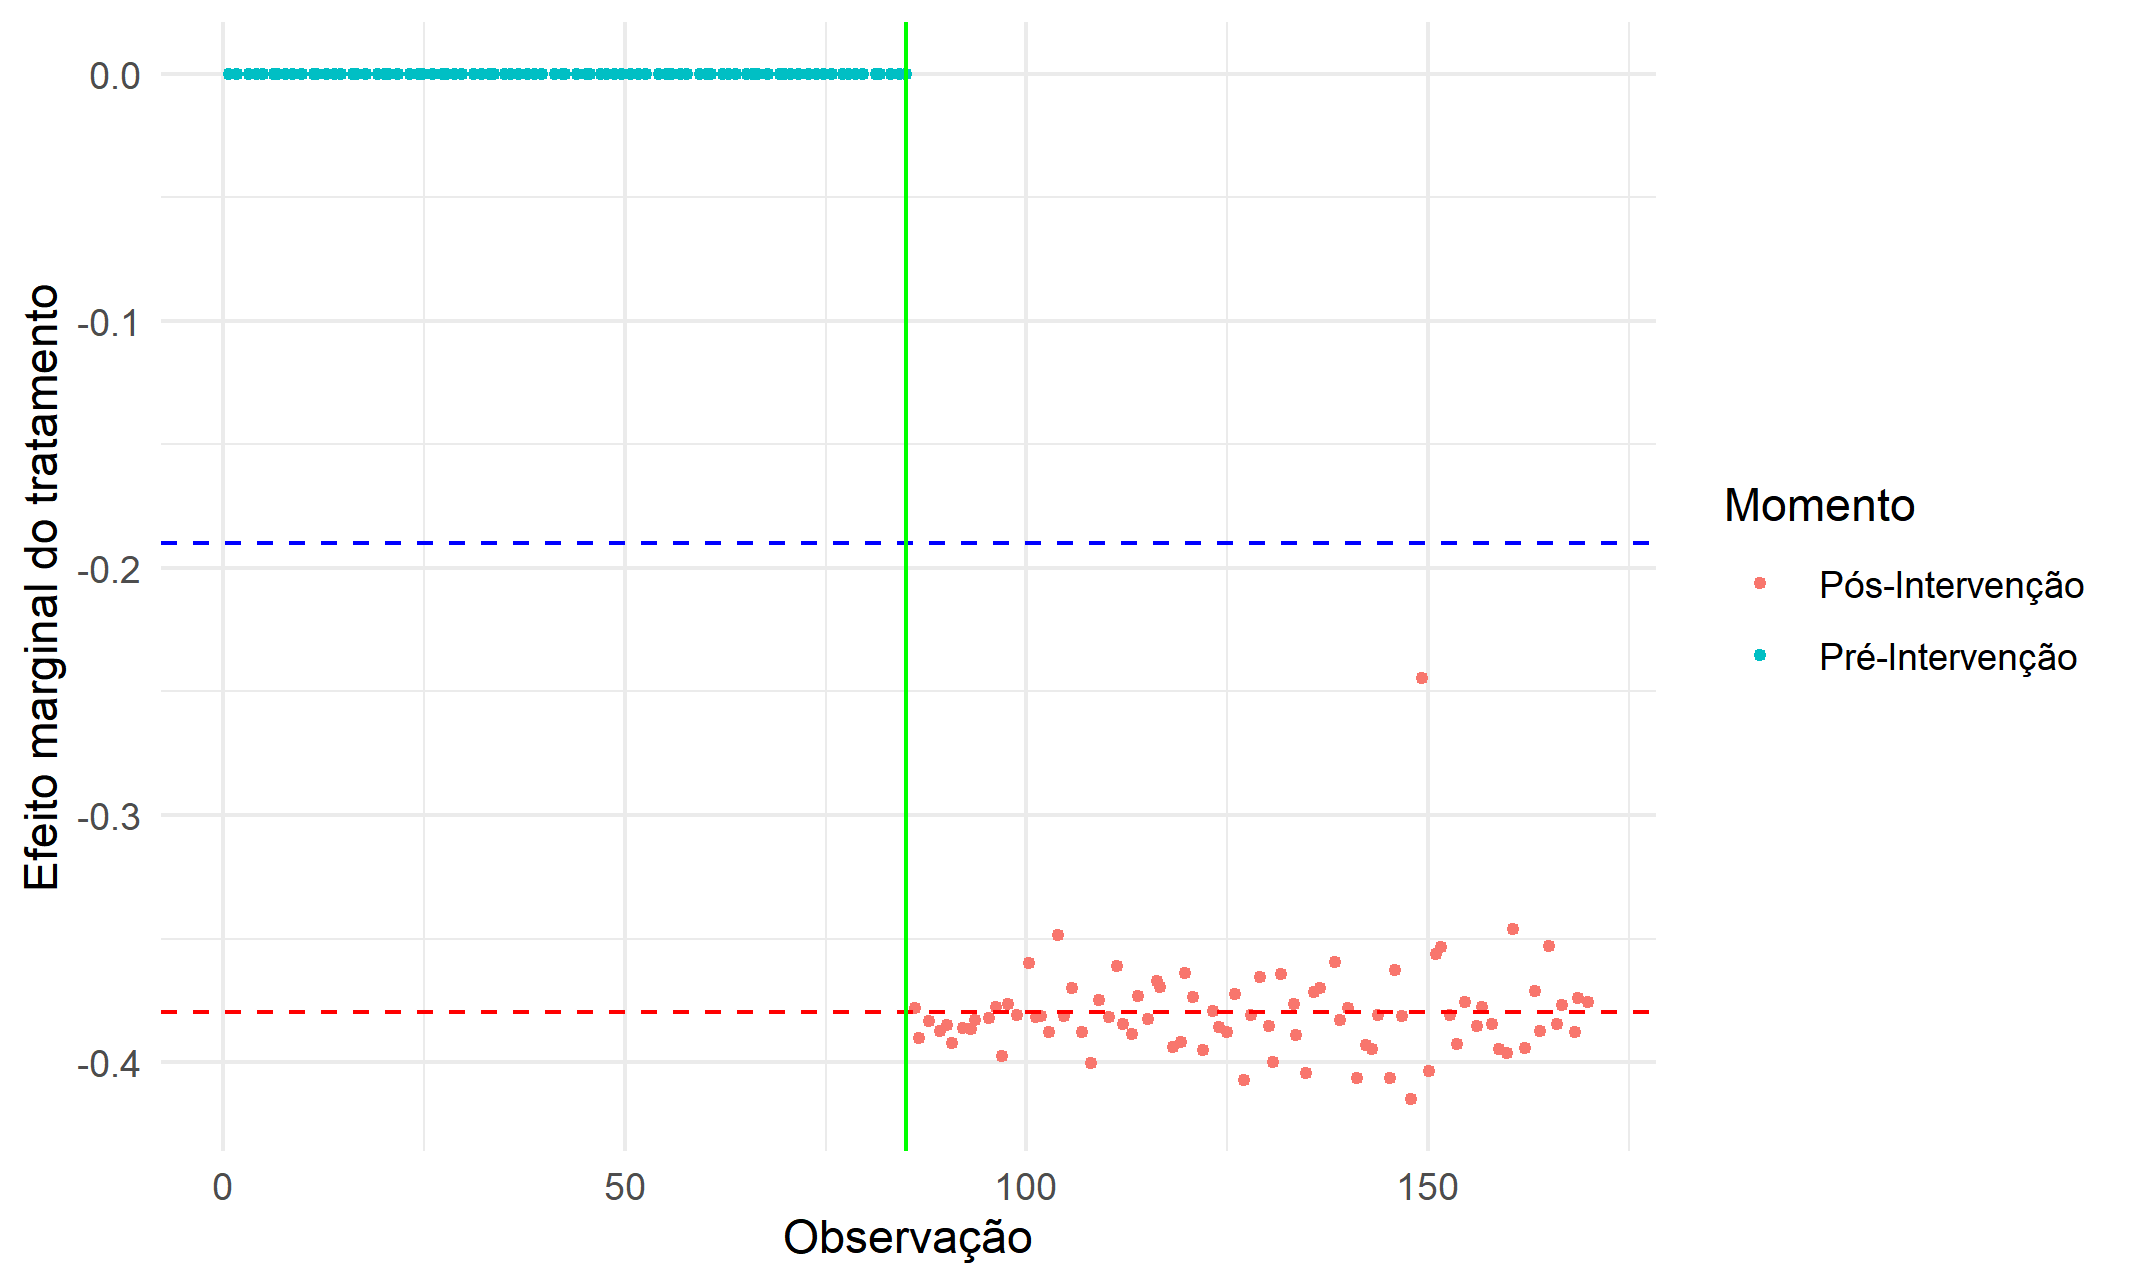
\includegraphics[width=0.7\linewidth]{"Figuras/Efeitos_marginais_2010_2013.png"} \\
\caption*{\RaggedRight Fonte: Elaboração própria à partir dos Microdados do ENADE disponíveis em \cite{INEP2020}.}
\end{figure}

Por outro lado, a educação da mãe ganhou significância estatística e apresentou um valor positivo relativamente elevado. Isso aliado à não significância estatística da variável de renda, talvez possa indicar que os cursos analisados no segundo ciclo possam ter uma composição estudantil diferentes dos cursos do primeiro ciclo.

Na seção seguinte, fez-se uma breve recapitulação do problema de pesquisa, dos passos tomados para a estimação e dos resultados e tecem-se as considerações finais sobre o trabalho, indicando possíveis caminhos futuros e aplicações.

\newpage 

\global\pdfpageattr\expandafter{\the\pdfpageattr/Rotate 90}
\begin{sidewaystable}[ht] \centering \scriptsize
  \caption{Efeito médio de tratamento sobre os tratados - Ciclo 2009-2012} 
  \label{tab:resultados_2009_2012} 
\begin{tabular}{@{\extracolsep{5pt}}lD{,}{,}{-3} D{,}{,}{-3} D{,}{,}{-3} D{,}{,}{-3} } 
\\[-1.8ex]\hline 
\hline \\[-1.8ex] 
 & \multicolumn{4}{c}{\textit{ Variável dependente:}} \\ 
\cline{2-5} 
\\[-1.8ex] & \multicolumn{4}{c}{log(nota média)} \\ \\
 & \multicolumn{1}{c}{Diff-diff} & \multicolumn{1}{c}{Diff-diff + FE} & \multicolumn{1}{c}{Diff-diff + FE + PSM (logit)} & \multicolumn{1}{c}{Diff-diff + FE + PSM (entropia)} \\ 
\hline \\[-1.8ex] 
 Constante & -0,193 &  &  &  \\ 
  & (1,375) &  &  &  \\ 
  & & & & \\ 
 Tratamento & -0,028 &  &  &  \\ 
  & (0,054) &  &  &  \\ 
  & & & & \\ 
 Pós-tratamento & -0,020 & -0,023 & -0,008 & -0,045 \\ 
  & (0,079) & (0,090) & (0,083) & (0,085) \\ 
  & & & & \\ 
 Idade média & 0,315^{***} & 0,606^{***} & 0,737^{***} & 0,681^{***} \\ 
  & (0,099) & (0,148) & (0,171) & (0,164) \\ 
  & & & & \\ 
 Idade média² & -0,005^{***} & -0,010^{***} & -0,013^{***} & -0,012^{***} \\ 
  & (0,002) & (0,003) & (0,004) & (0,003) \\ 
  & & & & \\ 
 Prop. brancos & 0,060 & -3,106^{***} & -3,370^{***} & -3,338^{***} \\ 
  & (0,103) & (0,663) & (0,709) & (0,709) \\ 
  & & & & \\ 
 Prop. casados & -1,427^{**} & -2,836^{***} & -2,074^{**} & -2,436^{**} \\ 
  & (0,586) & (0,965) & (1,018) & (1,035) \\ 
  & & & & \\ 
 Prop. homens & -0,004 & 0,475 & 0,201 & 0,301 \\ 
  & (0,275) & (0,393) & (0,418) & (0,404) \\ 
  & & & & \\ 
 Prop. Ensino Médio+ & -0,270 & -0,057 & -0,273 & -0,211 \\ 
  & (0,262) & (0,566) & (0,551) & (0,557) \\ 
  & & & & \\ 
 Prop. Renda até 3SM & -0,599^{***} & -1,113^{***} & -1,310^{***} & -1,184^{***} \\ 
  & (0,216) & (0,301) & (0,285) & (0,274) \\ 
  & & & & \\ 
 Diff-and-diff/Impacto & 0,010 & -0,044 & 0,002 & 0,006 \\ 
  & (0,075) & (0,057) & (0,052) & (0,053) \\ 
  & & & & \\ 
\hline \\[-1.8ex] 
Observações & \multicolumn{1}{c}{170} & \multicolumn{1}{c}{170} & \multicolumn{1}{c}{170} & \multicolumn{1}{c}{170} \\ 
R$^{2}$ & \multicolumn{1}{c}{0,183} &  &  &  \\ 
R$^{2}$ ajustado & \multicolumn{1}{c}{0,132} &  &  &  \\ 
Erro-padrão residual & \multicolumn{1}{c}{0,239 (df = 159)} &  &  &  \\ Estatística F & \multicolumn{1}{c}{3,563$^{***}$ (df = 10; 159)} & \multicolumn{1}{c}{8,605$^{***}$ (df = 9; 76)} & \multicolumn{1}{c}{9,071$^{***}$ (df = 9; 76)} & \multicolumn{1}{c}{8,719$^{***}$ (df = 9; 76)} \\ \hline 
\hline \\[-1.8ex] 
\textit{Nota:}  & \multicolumn{4}{r}{$^{*}$p$<$0,1; $^{**}$p$<$0,05; $^{***}$p$<$0,01} \\ \hline 
\end{tabular} 
\caption*{Fonte: Elaboração própria à partir dos Microdados do ENADE disponíveis em \cite{INEP2020}.}
\end{sidewaystable} 

% Table created by stargazer v.5.2.2 by Marek Hlavac, Harvard University. E-mail: hlavac at fas.harvard.edu
% Date and time: qua, nov 18, 2020 - 21:48:06
% Requires LaTeX packages: dcolumn rotating 
\begin{sidewaystable} \centering \scriptsize
  \caption{Efeito médio de tratamento sobre os tratados - Ciclo 2010-2013} 
  \label{tab:resultados_2010_2013} 
\begin{tabular}{@{\extracolsep{5pt}}lD{,}{,}{-3} D{,}{,}{-3} D{,}{,}{-3} D{,}{,}{-3} } 
\\[-1.8ex]\hline 
\hline \\[-1.8ex] 
 & \multicolumn{4}{c}{\textit{Variável dependente:}} \\ 
\cline{2-5} 
\\[-1.8ex] & \multicolumn{4}{c}{log(nota média)} \\ \\
 & \multicolumn{1}{c}{Diff-diff} & \multicolumn{1}{c}{Diff-diff + FE} & \multicolumn{1}{c}{Diff-diff + FE + PSM (logit)} & \multicolumn{1}{c}{Diff-diff + FE + PSM (entropia)} \\ 
\hline \\[-1.8ex] 
 Constante & 3,017^{***} &  &  &  \\ 
  & (0,379) &  &  &  \\ 
  & & & & \\ 
 Tratamento & -0,007 &  &  &  \\ 
  & (0,019) &  &  &  \\ 
  & & & & \\ 
 Pós-tratamento & 0,131^{***} & 0,091^{*} & 0,045 & 0,072 \\ 
  & (0,043) & (0,048) & (0,051) & (0,050) \\ 
  & & & & \\ 
 Idade média & 0,057^{**} & 0,142^{***} & 0,181^{*} & 0,130 \\ 
  & (0,025) & (0,045) & (0,098) & (0,089) \\ 
  & & & & \\ 
 Idade média² & -0,001^{***} & -0,003^{***} & -0,003 & -0,002 \\ 
  & (0,0004) & (0,001) & (0,002) & (0,002) \\ 
  & & & & \\ 
 Prop. brancos & 0,038 & -0,137 & -0,050 & -0,083 \\ 
  & (0,041) & (0,140) & (0,147) & (0,152) \\ 
  & & & & \\ 
 Prop. casados & -0,080 & 0,100 & -0,129 & -0,133 \\ 
  & (0,244) & (0,326) & (0,369) & (0,377) \\ 
  & & & & \\ 
 Prop. homens & 0,048 & 0,225 & 0,144 & 0,236 \\ 
  & (0,063) & (0,173) & (0,179) & (0,188) \\ 
  & & & & \\ 
 Prop. Ensino Médio+ & 0,248^{***} & 0,380^{***} & 0,325^{***} & 0,340^{***} \\ 
  & (0,081) & (0,117) & (0,121) & (0,126) \\ 
  & & & & \\ 
 Prop. Renda até 3SM & -0,021 & -0,043 & 0,051 & 0,012 \\ 
  & (0,064) & (0,078) & (0,088) & (0,088) \\ 
  & & & & \\ 
 Diff-and-diff/Impacto & -0,019 & -0,040^{*} & -0,046^{**} & -0,042^{**} \\ 
  & (0,027) & (0,020) & (0,019) & (0,020) \\ 
  & & & & \\ 
\hline \\[-1.8ex] 
Observações & \multicolumn{1}{c}{170} & \multicolumn{1}{c}{170} & \multicolumn{1}{c}{170} & \multicolumn{1}{c}{170} \\ 
R$^{2}$ & \multicolumn{1}{c}{0,577} &  &  &  \\ 
R$^{2}$ ajustado & \multicolumn{1}{c}{0,551} &  &  &  \\ 
Erro-padrão residual & \multicolumn{1}{c}{0,084 (df = 159)} &  &  &  \\ 
Estatística F & \multicolumn{1}{c}{21,706$^{***}$ (df = 10; 159)} & \multicolumn{1}{c}{26,009$^{***}$ (df = 9; 76)} & \multicolumn{1}{c}{26,288$^{***}$ (df = 9; 76)} & \multicolumn{1}{c}{24,104$^{***}$ (df = 9; 76)} \\ 
\hline 
\hline \\[-1.8ex] 
\textit{Nota:}  & \multicolumn{4}{r}{$^{*}$p$<$0,1; $^{**}$p$<$0,05; $^{***}$p$<$0,01} \\ \hline \\
\end{tabular} 
\caption*{Fonte: Elaboração própria à partir dos Microdados do ENADE disponíveis em \cite{INEP2020}.}
\end{sidewaystable} 

\chapter{Conclusões}

\global\pdfpageattr\expandafter{\the\pdfpageattr/Rotate 0}

O intuito do presente trabalho era verificar se a greve federal de 2012 das instituições de ensino superior teve algum efeito sobre o desempenho dos discentes na prova do ENADE, tanto daquele ano quanto de 2013. Para tanto, empregaram-se, inicialmente, métodos de pareamento, visando deixar os grupos de tratamento e controle o mais parecidos possível. Tendo sido feito isso, procedeu-se a estimação do modelo utilizado Diferenças-em-Diferenças com controle de efeitos fixos individuais de cada IES. 

Os resultados mostram que no ano da greve, 2012, o seu efeito sobre as notas médias das instituições não foi significativo, muito provavelmente pelo pequeno intervalo de tempo entre o final da greve e a prova. Por outro lado, ao se analisar a prova do ano seguinte, 2013, obteve-se um impacto negativo estatisticamente significativo, apontando para a existência de um efeito deletério não-contemporâneo da greve sobre o desempenho dos discentes.

Novos trabalhos devem buscar dados mais específicos sobre as greves, como a duração dela em cada instituição, possibilitando assim a criação de uma variável que capture a intensidade do tratamento. Além disso, uma vez que as IES que escolheram aderir ao movimento grevista têm características distintas das demais, seria interessante utilizar a correção de \citeonline{Heckman1979}, visando modelar a equação de autosseleção das instituições.

\postextual

\bibliography{referencias.bib}

\begin{flushleft} \chapter{Apêndice} \end{flushleft}

\section{Lista de instituições de ensino superior utilizadas na estimação}

% Table created by stargazer v.5.2.2 by Marek Hlavac, Harvard University. E-mail: hlavac at fas.harvard.edu
% Date and time: qui, nov 19, 2020 - 16:25:22
% Requires LaTeX packages: dcolumn 
{\tiny
\begin{center}
\begin{longtable}[H]{ll}  
   \caption{Lista de instituições de ensino superior com dummy de aderência à greve}
  \label{tab:lista_de_ies} \\
  
   \multicolumn{1}{l}{\textbf{Nome}} & \multicolumn{1}{l}{\textbf{Aderiram}}  \\ \hline 
\endfirsthead

\multicolumn{2}{c}%
{{\bfseries \tablename\ \thetable{} -- continuação da página anterior}} \\
 \multicolumn{1}{l}{\textbf{Nome}} & \multicolumn{1}{l}{\textbf{Aderiram}} \\ \hline 
\endhead

\hline \multicolumn{2}{r}{{Continua na próxima página}} \\ \hline
\endfoot

\\ \hline \\ \caption*{\RaggedRight Fonte: Elaboração própria à partir dos Microdados do ENADE disponíveis em \cite{INEP2020}.}
\endlastfoot
\hline \\[-1.8ex] 
\multicolumn{1}{l}{UNIVERSIDADE FEDERAL DE MATO GROSSO} & \multicolumn{1}{l}{Não} \\ 
\multicolumn{1}{l}{UNIVERSIDADE DE BRASILIA} & \multicolumn{1}{l}{Não} \\ 
\multicolumn{1}{l}{UNIVERSIDADE FEDERAL DE SERGIPE} & \multicolumn{1}{l}{Sim} \\ 
\multicolumn{1}{l}{UNIVERSIDADE FEDERAL DO AMAZONAS} & \multicolumn{1}{l}{Sim} \\ 
\multicolumn{1}{l}{UNIVERSIDADE FEDERAL DO PIAUI} & \multicolumn{1}{l}{Sim} \\ 
\multicolumn{1}{l}{UNIVERSIDADE FEDERAL DE OURO PRETO} & \multicolumn{1}{l}{Sim} \\ 
\multicolumn{1}{l}{UNIVERSIDADE FEDERAL DE SAO CARLOS} & \multicolumn{1}{l}{Sim} \\ 
\multicolumn{1}{l}{UNIVERSIDADE FEDERAL DE VICOSA} & \multicolumn{1}{l}{Sim} \\ 
\multicolumn{1}{l}{UNIVERSIDADE ESTADUAL DE LONDRINA} & \multicolumn{1}{l}{Não} \\ 
\multicolumn{1}{l}{UNIVERSIDADE FEDERAL DO RIO GRANDE} & \multicolumn{1}{l}{Sim} \\ 
\multicolumn{1}{l}{UNIVERSIDADE FEDERAL DE UBERLANDIA} & \multicolumn{1}{l}{Sim} \\ 
\multicolumn{1}{l}{UNIVERSIDADE ESTADUAL DE SANTA CRUZ} & \multicolumn{1}{l}{Não} \\ 
\multicolumn{1}{l}{UNIVERSIDADE ESTADUAL DO CEARA} & \multicolumn{1}{l}{Não} \\ 
\multicolumn{1}{l}{UNIVERSIDADE DO ESTADO DA BAHIA} & \multicolumn{1}{l}{Não} \\ 
\multicolumn{1}{l}{FUNDACAO UNIVERSIDADE DO ESTADO DE SANTA CATARINA} & \multicolumn{1}{l}{Não} \\ 
\multicolumn{1}{l}{UNIVERSIDADE ESTADUAL DE GOIAS} & \multicolumn{1}{l}{Não} \\ 
\multicolumn{1}{l}{UNIVERSIDADE ESTADUAL PAULISTA JULIO DE MESQUITA FILHO} & \multicolumn{1}{l}{Não} \\ 
\multicolumn{1}{l}{UNIVERSIDADE ESTADUAL DE MARINGA} & \multicolumn{1}{l}{Não} \\ 
\multicolumn{1}{l}{UNIVERSIDADE DO ESTADO DO RIO GRANDE DO NORTE} & \multicolumn{1}{l}{Não} \\ 
\multicolumn{1}{l}{UNIVERSIDADE ESTADUAL DO VALE DO ACARAU} & \multicolumn{1}{l}{Não} \\ 
\multicolumn{1}{l}{UNIVERSIDADE FEDERAL DE SAO JOAO DEL REI} & \multicolumn{1}{l}{Sim} \\ 
\multicolumn{1}{l}{UNIVERSIDADE ESTADUAL DE MONTES CLAROS} & \multicolumn{1}{l}{Não} \\ 
\multicolumn{1}{l}{UNIVERSIDADE DE PERNAMBUCO} & \multicolumn{1}{l}{Não} \\ 
\multicolumn{1}{l}{UNIVERSIDADE DO ESTADO DO RIO DE JANEIRO} & \multicolumn{1}{l}{Não} \\ 
\multicolumn{1}{l}{UNIVERSIDADE FEDERAL DO MARANHAO} & \multicolumn{1}{l}{Sim} \\ 
\multicolumn{1}{l}{UNIVERSIDADE ESTADUAL DA PARAIBA} & \multicolumn{1}{l}{Não} \\ 
\multicolumn{1}{l}{UNIVERSIDADE ESTADUAL DO MARANHAO} & \multicolumn{1}{l}{Não} \\ 
\multicolumn{1}{l}{UNIVERSIDADE FEDERAL DO PARA} & \multicolumn{1}{l}{Sim} \\ 
\multicolumn{1}{l}{UNIVERSIDADE FEDERAL DO RIO GRANDE DO NORTE} & \multicolumn{1}{l}{Não} \\ 
\multicolumn{1}{l}{UNIVERSIDADE FEDERAL DO PARANA} & \multicolumn{1}{l}{Sim} \\ 
\multicolumn{1}{l}{UNIVERSIDADE FEDERAL FLUMINENSE} & \multicolumn{1}{l}{Sim} \\ 
\multicolumn{1}{l}{UNIVERSIDADE FEDERAL DO ESPIRITO SANTO} & \multicolumn{1}{l}{Sim} \\ 
\multicolumn{1}{l}{UNIVERSIDADE FEDERAL RURAL DO RIO DE JANEIRO} & \multicolumn{1}{l}{Sim} \\ 
\multicolumn{1}{l}{UNIVERSIDADE FEDERAL DE MINAS GERAIS} & \multicolumn{1}{l}{Sim} \\ 
\multicolumn{1}{l}{UNIVERSIDADE FEDERAL DE JUIZ DE FORA} & \multicolumn{1}{l}{Sim} \\ 
\multicolumn{1}{l}{UNIVERSIDADE FEDERAL DE ALAGOAS} & \multicolumn{1}{l}{Sim} \\ 
\multicolumn{1}{l}{UNIVERSIDADE FEDERAL DA BAHIA} & \multicolumn{1}{l}{Sim} \\ 
\multicolumn{1}{l}{UNIVERSIDADE FEDERAL DA PARAIBA} & \multicolumn{1}{l}{Sim} \\ 
\multicolumn{1}{l}{UNIVERSIDADE FEDERAL DE PERNAMBUCO} & \multicolumn{1}{l}{Sim} \\ 
\multicolumn{1}{l}{UNIVERSIDADE FEDERAL DO RIO GRANDE DO SUL} & \multicolumn{1}{l}{Sim} \\ 
\multicolumn{1}{l}{UNIVERSIDADE FEDERAL DE SANTA MARIA} & \multicolumn{1}{l}{Sim} \\ 
\multicolumn{1}{l}{UNIVERSIDADE FEDERAL DO CEARA} & \multicolumn{1}{l}{Sim} \\ 
\multicolumn{1}{l}{UNIVERSIDADE FEDERAL DE GOIAS} & \multicolumn{1}{l}{Sim} \\ 
\multicolumn{1}{l}{UNIVERSIDADE FEDERAL DE SANTA CATARINA} & \multicolumn{1}{l}{Não} \\ 
\multicolumn{1}{l}{UNIVERSIDADE FEDERAL DO RIO DE JANEIRO} & \multicolumn{1}{l}{Sim} \\ 
\multicolumn{1}{l}{UNIVERSIDADE FEDERAL RURAL DE PERNAMBUCO} & \multicolumn{1}{l}{Sim} \\ 
\multicolumn{1}{l}{UNIVERSIDADE TECNOLOGICA FEDERAL DO PARANA} & \multicolumn{1}{l}{Não} \\ 
\multicolumn{1}{l}{UNIVERSIDADE FEDERAL RURAL DO SEMIARIDO} & \multicolumn{1}{l}{Não} \\ 
\multicolumn{1}{l}{UNIVERSIDADE FEDERAL DE LAVRAS} & \multicolumn{1}{l}{Sim} \\ 
\multicolumn{1}{l}{CENTRO FEDERAL DE EDUCACAO TECNOLOGICA CELSO SUCKOW DA FONSECA} & \multicolumn{1}{l}{Sim} \\ 
\multicolumn{1}{l}{UNIVERSIDADE FEDERAL DOS VALES DO JEQUITINHONHA E MUCURI} & \multicolumn{1}{l}{Sim} \\ 
\multicolumn{1}{l}{INSTITUTO FEDERAL DE EDUCACAO, CIENCIA E TECNOLOGIA DA BAHIA} & \multicolumn{1}{l}{Não} \\ 
\multicolumn{1}{l}{UNIVERSIDADE ESTADUAL DO OESTE DO PARANA} & \multicolumn{1}{l}{Não} \\ 
\multicolumn{1}{l}{UNIVERSIDADE FEDERAL DE PELOTAS} & \multicolumn{1}{l}{Sim} \\ 
\multicolumn{1}{l}{UNIVERSIDADE ESTADUAL DE FEIRA DE SANTANA} & \multicolumn{1}{l}{Não} \\ 
\multicolumn{1}{l}{UNIVERSIDADE ESTADUAL DO SUDOESTE DA BAHIA} & \multicolumn{1}{l}{Não} \\ 
\multicolumn{1}{l}{UNIVERSIDADE FEDERAL DO ESTADO DO RIO DE JANEIRO} & \multicolumn{1}{l}{Sim} \\ 
\multicolumn{1}{l}{UNIVERSIDADE FEDERAL DE MATO GROSSO DO SUL} & \multicolumn{1}{l}{Não} \\ 
\multicolumn{1}{l}{FUNDACAO UNIVERSIDADE FEDERAL DE RONDONIA} & \multicolumn{1}{l}{Sim} \\ 
\multicolumn{1}{l}{UNIVERSIDADE DO ESTADO DE MATO GROSSO} & \multicolumn{1}{l}{Não} \\ 
\multicolumn{1}{l}{UNIVERSIDADE ESTADUAL DE PONTA GROSSA} & \multicolumn{1}{l}{Não} \\ 
\multicolumn{1}{l}{UNIVERSIDADE ESTADUAL DO PIAUI} & \multicolumn{1}{l}{Não} \\ 
\multicolumn{1}{l}{UNIVERSIDADE FEDERAL DE RORAIMA} & \multicolumn{1}{l}{Sim} \\ 
\multicolumn{1}{l}{UNIVERSIDADE DO TOCANTINS} & \multicolumn{1}{l}{Não} \\ 
\multicolumn{1}{l}{UNIVERSIDADE ESTADUAL DE MATO GROSSO DO SUL} & \multicolumn{1}{l}{Não} \\ 
\multicolumn{1}{l}{UNIVERSIDADE ESTADUAL DO CENTRO OESTE} & \multicolumn{1}{l}{Não} \\ 
\multicolumn{1}{l}{INSTITUTO FEDERAL DE EDUCACAO, CIENCIA E TECNOLOGIA DA PARAIBA} & \multicolumn{1}{l}{Sim} \\ 
\multicolumn{1}{l}{UNIVERSIDADE FEDERAL DE CAMPINA GRANDE} & \multicolumn{1}{l}{Sim} \\ 
\multicolumn{1}{l}{UNIVERSIDADE DO ESTADO DO AMAZONAS} & \multicolumn{1}{l}{Não} \\ 
\multicolumn{1}{l}{INSTITUTO FEDERAL DE EDUCACAO, CIENCIA E TECNOLOGIA DO NORTE DE MINAS GERAIS} & \multicolumn{1}{l}{Não} \\ 
\multicolumn{1}{l}{INSTITUTO FEDERAL DE EDUCACAO, CIENCIA E TECNOLOGIA DE MINAS GERAIS} & \multicolumn{1}{l}{Sim} \\ 
\multicolumn{1}{l}{UNIVERSIDADE ESTADUAL DO RIO GRANDE DO SUL} & \multicolumn{1}{l}{Não} \\ 
\multicolumn{1}{l}{FUNDACAO UNIVERSIDADE FEDERAL DO TOCANTINS} & \multicolumn{1}{l}{Sim} \\ 
\multicolumn{1}{l}{FUNDACAO UNIVERSIDADE FEDERAL DO VALE DO SAO FRANCISCO} & \multicolumn{1}{l}{Sim} \\ 
\multicolumn{1}{l}{FUNDACAO UNIVERSIDADE FEDERAL DA GRANDE DOURADOS} & \multicolumn{1}{l}{Sim} \\ 
\multicolumn{1}{l}{UNIVERSIDADE ESTADUAL DE RORAIMA} & \multicolumn{1}{l}{Não} \\ 
\multicolumn{1}{l}{UNIVERSIDADE ESTADUAL DE ALAGOAS UNEAL} & \multicolumn{1}{l}{Não} \\ 
\multicolumn{1}{l}{FUNDACAO UNIVERSIDADE FEDERAL DO PAMPA UNIPAMPA} & \multicolumn{1}{l}{Não} \\ 
\multicolumn{1}{l}{UNIVERSIDADE FEDERAL DO ACRE} & \multicolumn{1}{l}{Sim} \\ 
\multicolumn{1}{l}{UNIVERSIDADE REGIONAL DO CARIRI} & \multicolumn{1}{l}{Não} \\ 
\multicolumn{1}{l}{UNIVERSIDADE FEDERAL DO AMAPA} & \multicolumn{1}{l}{Sim} \\ 
\multicolumn{1}{l}{UNIVERSIDADE FEDERAL DO RECONCAVO DA BAHIA} & \multicolumn{1}{l}{Sim} \\ 
\multicolumn{1}{l}{UNIVERSIDADE FEDERAL DE SAO PAULO} & \multicolumn{1}{l}{Sim} \\ 
\multicolumn{1}{l}{UNIVERSIDADE FEDERAL DO TRIANGULO MINEIRO} & \multicolumn{1}{l}{Sim} \\ 
\multicolumn{1}{l}{INSTITUTO FEDERAL DE EDUCACAO, CIENCIA E TECNOLOGIA DO PIAUI} & \multicolumn{1}{l}{Sim} \\[-1.8ex] 
\end{longtable}
\end{center}
}

\section{Balanceamento das covariadas - Testes de placebo}

\begin{figure}[H]
	\centering
	\caption{Balanceamento das covariadas - Ciclo 2009-2012 - Teste de placebo 1}
	\label{fig:balanceamento_covariadas_2009_2012_placebo_1}
	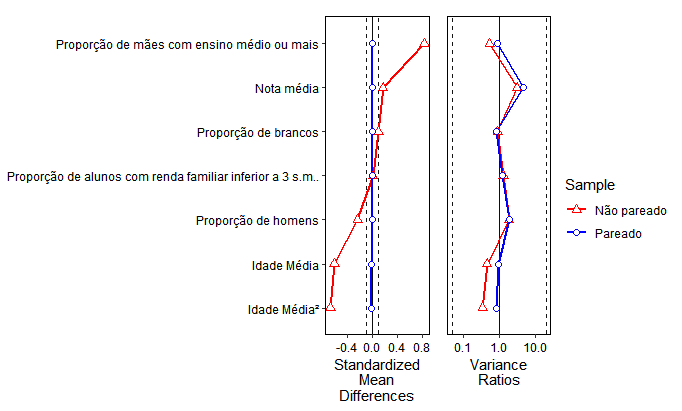
\includegraphics[width=0.7\linewidth]{"Figuras/balanceamento_covariadas_2009_2012_placebo1.png"}
	\caption*{\RaggedRight Fonte: Elaboração própria à partir dos Microdados do ENADE disponíveis em \cite{INEP2020}.}
\end{figure}

\begin{figure}[H]
	\centering
	\caption{Balanceamento das covariadas - Ciclo 2009-2012 - Teste de placebo 2}
	\label{fig:balanceamento_covariadas_2009_2012_placebo_2}
	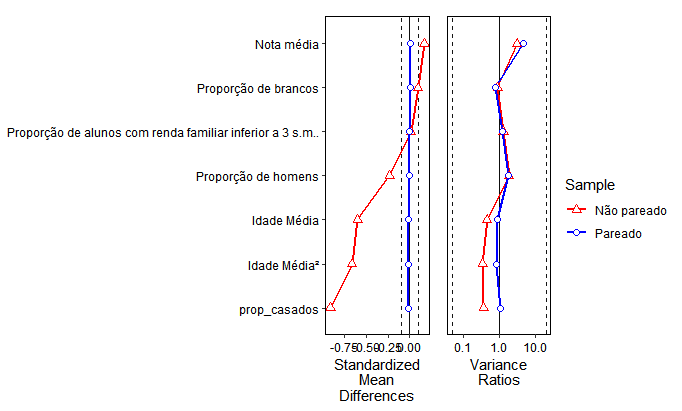
\includegraphics[width=0.7\linewidth]{"Figuras/balanceamento_covariadas_2009_2012_placebo2.png"}
\caption*{\RaggedRight Fonte: Elaboração própria à partir dos Microdados do ENADE disponíveis em \cite{INEP2020}.}
\end{figure}

\begin{figure}[H]
	\centering
	\caption{Balanceamento das covariadas - Ciclo 2010-2013 - Teste de placebo 1}
	\label{fig:balanceamento_covariadas_2010_2013_placebo_1}
	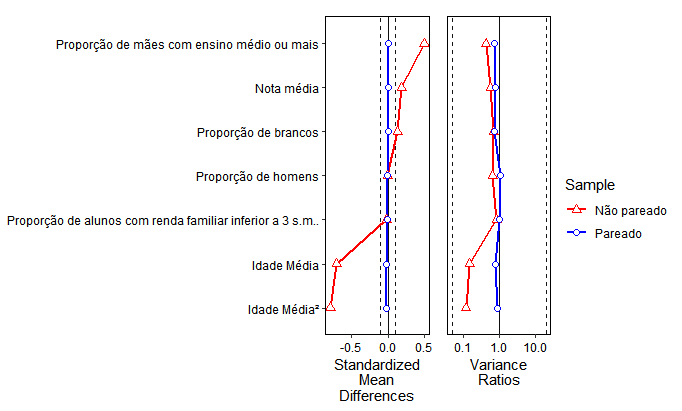
\includegraphics[width=0.7\linewidth]{"Figuras/balanceamento_covariadas_2010_2013_placebo1.png"}
	\caption*{\RaggedRight Fonte: Elaboração própria à partir dos Microdados do ENADE disponíveis em \cite{INEP2020}.}
\end{figure}

\begin{figure}[H]
	\centering
	\caption{Balanceamento das covariadas - Ciclo 2010-2013 - Teste de placebo 2}
	\label{fig:balanceamento_covariadas_2010_2013_placebo_2}
	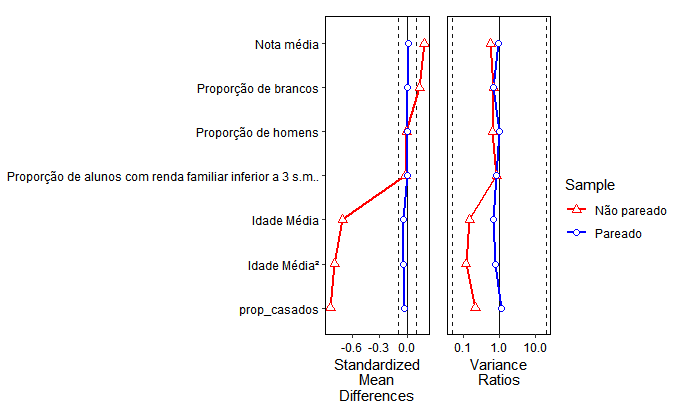
\includegraphics[width=0.7\linewidth]{"Figuras/balanceamento_covariadas_2010_2013_placebo2.png"}
	\caption*{\RaggedRight Fonte: Elaboração própria à partir dos Microdados do ENADE disponíveis em \cite{INEP2020}.}
\end{figure}

\end{document}
